\documentclass[a4paper,12pt]{report}
\usepackage[utf8]{inputenc}  
\usepackage[T1]{fontenc}    
\usepackage[french]{babel}   
\usepackage{pdfpages}
\usepackage{xcolor,graphicx}
\usepackage{amsmath}
\usepackage{subcaption}
\usepackage{float} 
\usepackage[top=0.6in,bottom=0.6in,right=1in,left=1in]{geometry}
\usepackage{changepage}
\usepackage{acronym}
\usepackage{setspace}
\usepackage{amssymb}    
\usepackage{microtype}   
\usepackage{algorithm}   
\usepackage{algorithmic}   
\usepackage[hidelinks, pdfencoding=auto]{hyperref}   

  
\newcommand{\frontmatter}{  
    \pagenumbering{arabic}  
      \setcounter{page}{1}  
}

\newcommand{\mainmatter}{  
    \pagenumbering{arabic}  
    \setcounter{page}{1}  
}

\newcommand{\mychapter}[2]{  
    \chapter{#1}  
    \markboth{#2}{#2}  
}

  
\setlength{\intextsep}{10pt}     
\setlength{\textfloatsep}{10pt}   


\newenvironment{fquote}
  {\begin{quote}\itshape}
  {\end{quote}}

  
\addto\captionsfrench{  
  \renewcommand{\contentsname}{Table des matières}  
  \renewcommand{\listfigurename}{Liste des figures}  
  \renewcommand{\listtablename}{Liste des tableaux}  
}

\begin{document}
\sloppy

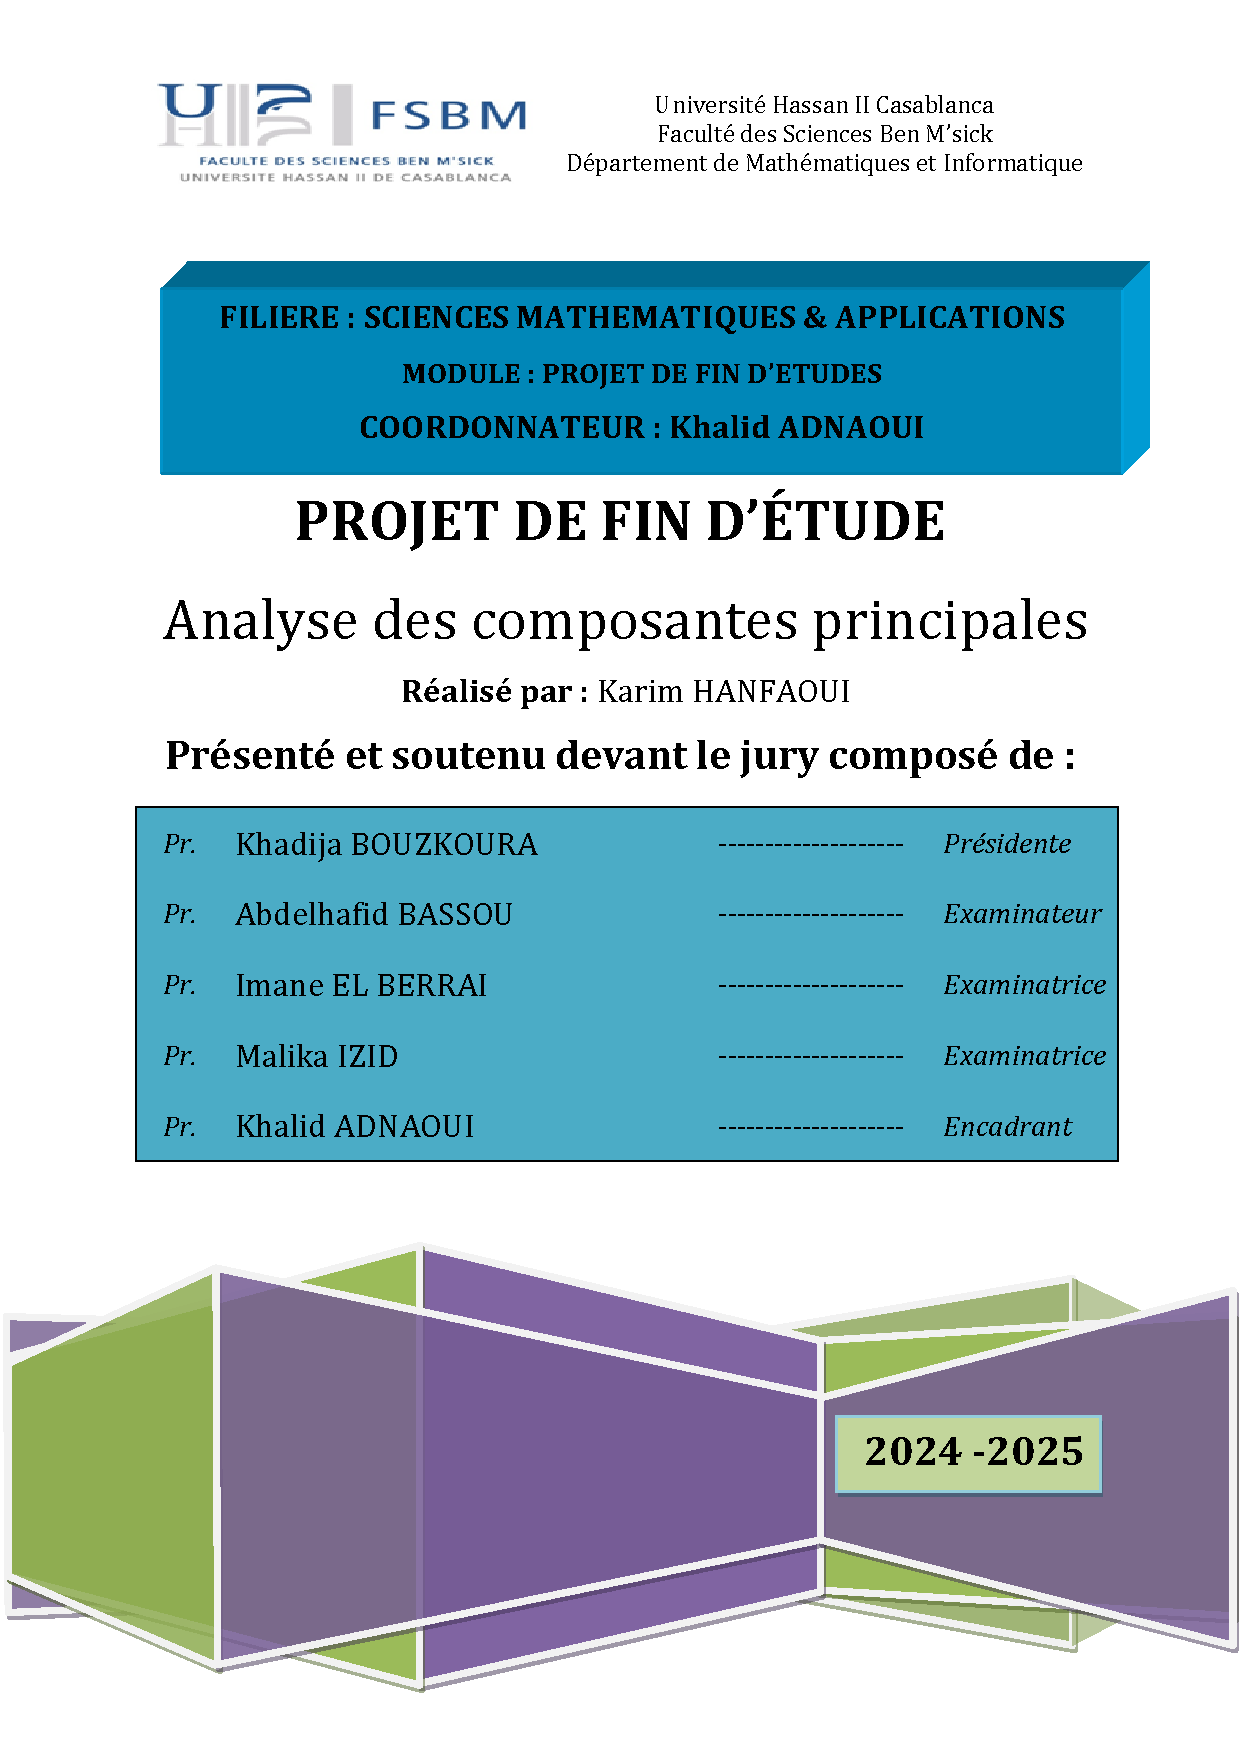
\includepdf[pages=1]{karim_page.pdf}

\frontmatter    
\tableofcontents
\listoftables
\listoffigures

\mainmatter    

\chapter{Remerciement}

\begin{center}
  \textit{Chers membres du jury,}
\end{center}

\vspace{0.5cm}

\onehalfspacing
Je tiens à vous remercier sincèrement pour votre présence et votre attention lors de ma soutenance de projet de fin d’étude. Cet aboutissement n’aurait pas été possible sans votre soutien et vos conseils tout au long de cette aventure.

\vspace{0.3cm}
Je souhaite également remercier Pr. ADNAOUI Khalid pour leur collaboration et leur engagement dans ce projet et leur patient avec moi. \textit{Nous avons travaillé ensemble avec passion et détermination pour offrir un travail de qualité.}
\vspace{0.3cm}

Je tiens également à exprimer ma gratitude envers mes enseignants qui m’ont éclairé de leur expertise et ont contribué à l’élaboration de ce projet. \textit{Vous avez été d’une grande aide dans mon parcours académique et professionnel.}
\vspace{0.3cm} \\
\textit{Enfin, je voudrais adresser un grand merci à ma famille et mes amis qui m’ont soutenu et encouragé tout au long de cette longue période d’étude. Votre amour constant m’a motivé à aller de l’avant malgré les défis.}
\vspace{0.3cm}
Encore une fois, merci infiniment pour votre temps, votre soutien et l’opportunité de présenter mon projet devant vous. Cela restera un moment inoubliable de ma vie.
\vspace{0.5cm}

\begin{flushright}
  \textbf{Cordialement,} \\
  \vspace{0.2cm}
  \textit{HANFAOUI Karim}
\end{flushright}


\newpage
\mychapter{Introduction Générale}{Introduction Générale}

L'Analyse des Composantes Principales (ACP) est une méthode statistique de réduction de dimensionnalité qui transforme des variables corrélées en un ensemble de composantes orthogonales maximisant la variance expliquée. Fondée sur l'algèbre linéaire et la théorie des matrices, elle permet d'extraire l'information essentielle tout en préservant la structure des données.

\section{Applications pratiques}
\begin{itemize}
    \item \textbf{Génomique} : Analyse de l'expression génique et classification d'échantillons biologiques
    \item \textbf{Finance} : Identification des facteurs de risque dans les portefeuilles d'investissement
    \item \textbf{Imagerie numérique} : Compression d'images et reconnaissance faciale (méthode Eigenfaces)
    \item \textbf{Météorologie} : Détection des modes climatiques dominants (ex: El Niño)
\end{itemize}

\section{Contexte historique}
\begin{itemize}
    \item 1901 : Karl Pearson établit les bases mathématiques
    \item 1933 : Harold Hotelling formalise la méthode moderne
    \item 1960s : Applications en psychométrie et économétrie
    \item 2000s : Intégration dans l'apprentissage automatique
\end{itemize}

\section{Cas classiques d'utilisation}
\begin{itemize}
    \item \textbf{Reconnaissance faciale (Eigenfaces)} : 
    Réduction de 10 000 pixels à 150 composantes principales tout en conservant 95\  
    
    \item \textbf{Analyse génomique} : 
    Visualisation de populations humaines à partir de 500 000 SNPs (Polymorphismes nucléotidiques)
    
    \item \textbf{Marchés financiers} : 
    Identification de 3 facteurs principaux expliquant 80\  
    
    \item \textbf{Études de consommation} : 
    Réduction de 50 variables marketing en 2 axes principaux : "praticité" vs "luxe"
    
    \item \textbf{Climatologie} : 
    Détection du phénomène El Niño à partir de 40 ans de données océanographiques multidimensionnelles
\end{itemize}

\subsection{Simulation et m\'ethodologie}
Nous simulons les donn\'ees de 1000 passagers normaux et 20 passagers suspects \`a l'aide de distributions gaussiennes multivariées. Chaque observation est un vecteur \`a 4 dimensions. Les donn\'ees sont ensuite standardis\'ees, projet\'ees en 2D via l'ACP, puis soumises \`a l'algorithme \textit{Isolation Forest} pour d\'etecter les anomalies.

\subsection{R\'esultats}

\subsubsection{Projection en deux dimensions par ACP}
\begin{figure}[H]
  \centering
  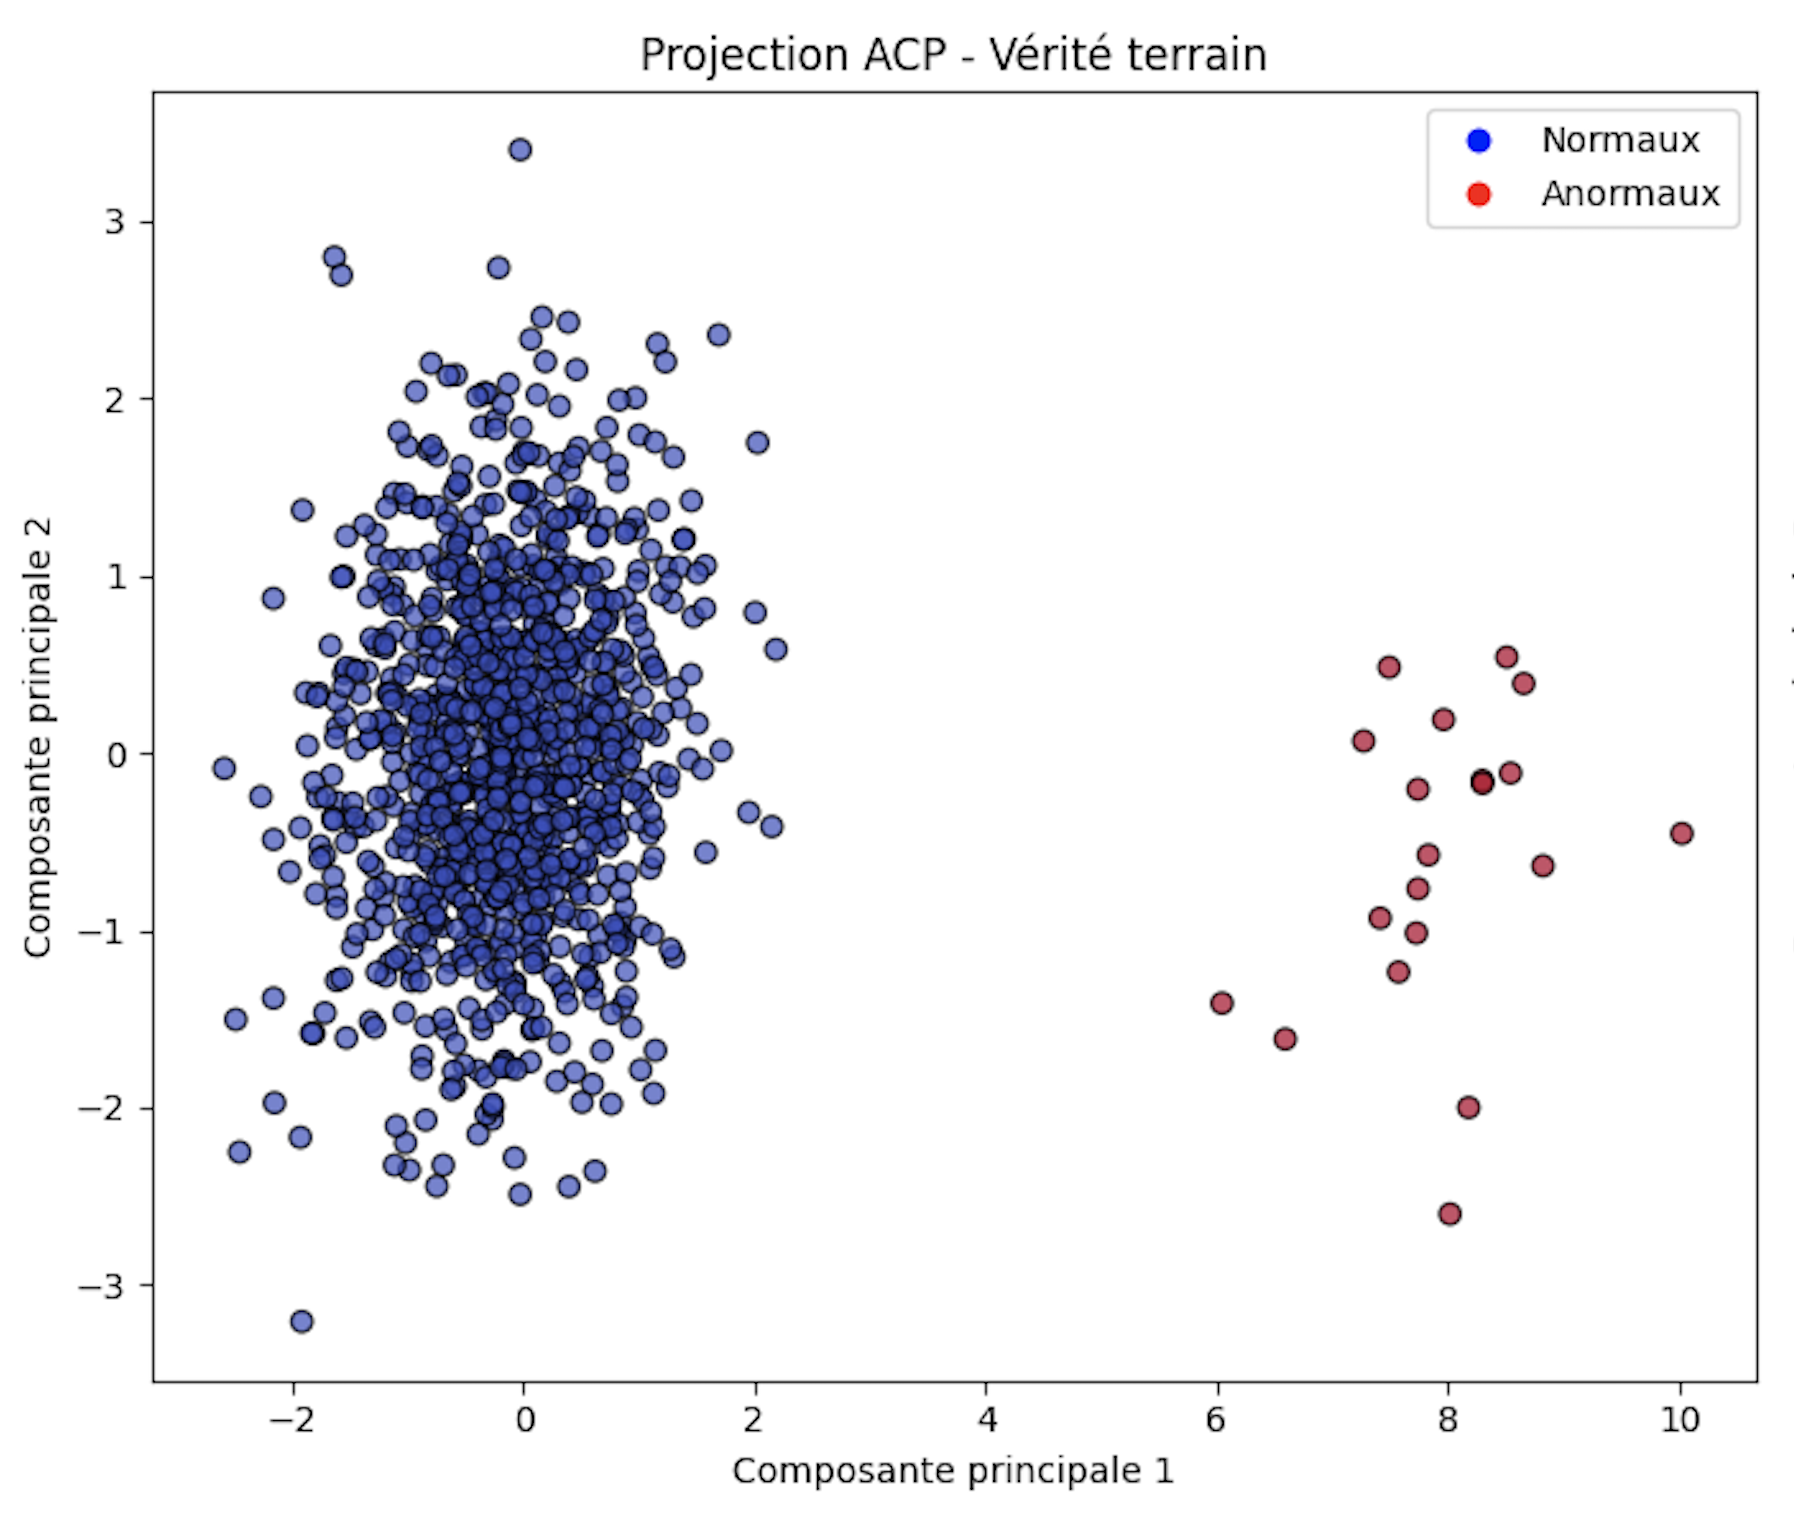
\includegraphics[width=0.8\textwidth]{projection_verite.png}
  \caption{Projection ACP - V\'erite terrain : les passagers normaux sont en bleu, les suspects simul\'es en rouge.}
  \label{fig:verite}
\end{figure}

\subsubsection{D\'etection automatique des comportements anormaux}
\begin{figure}[H]
  \centering
  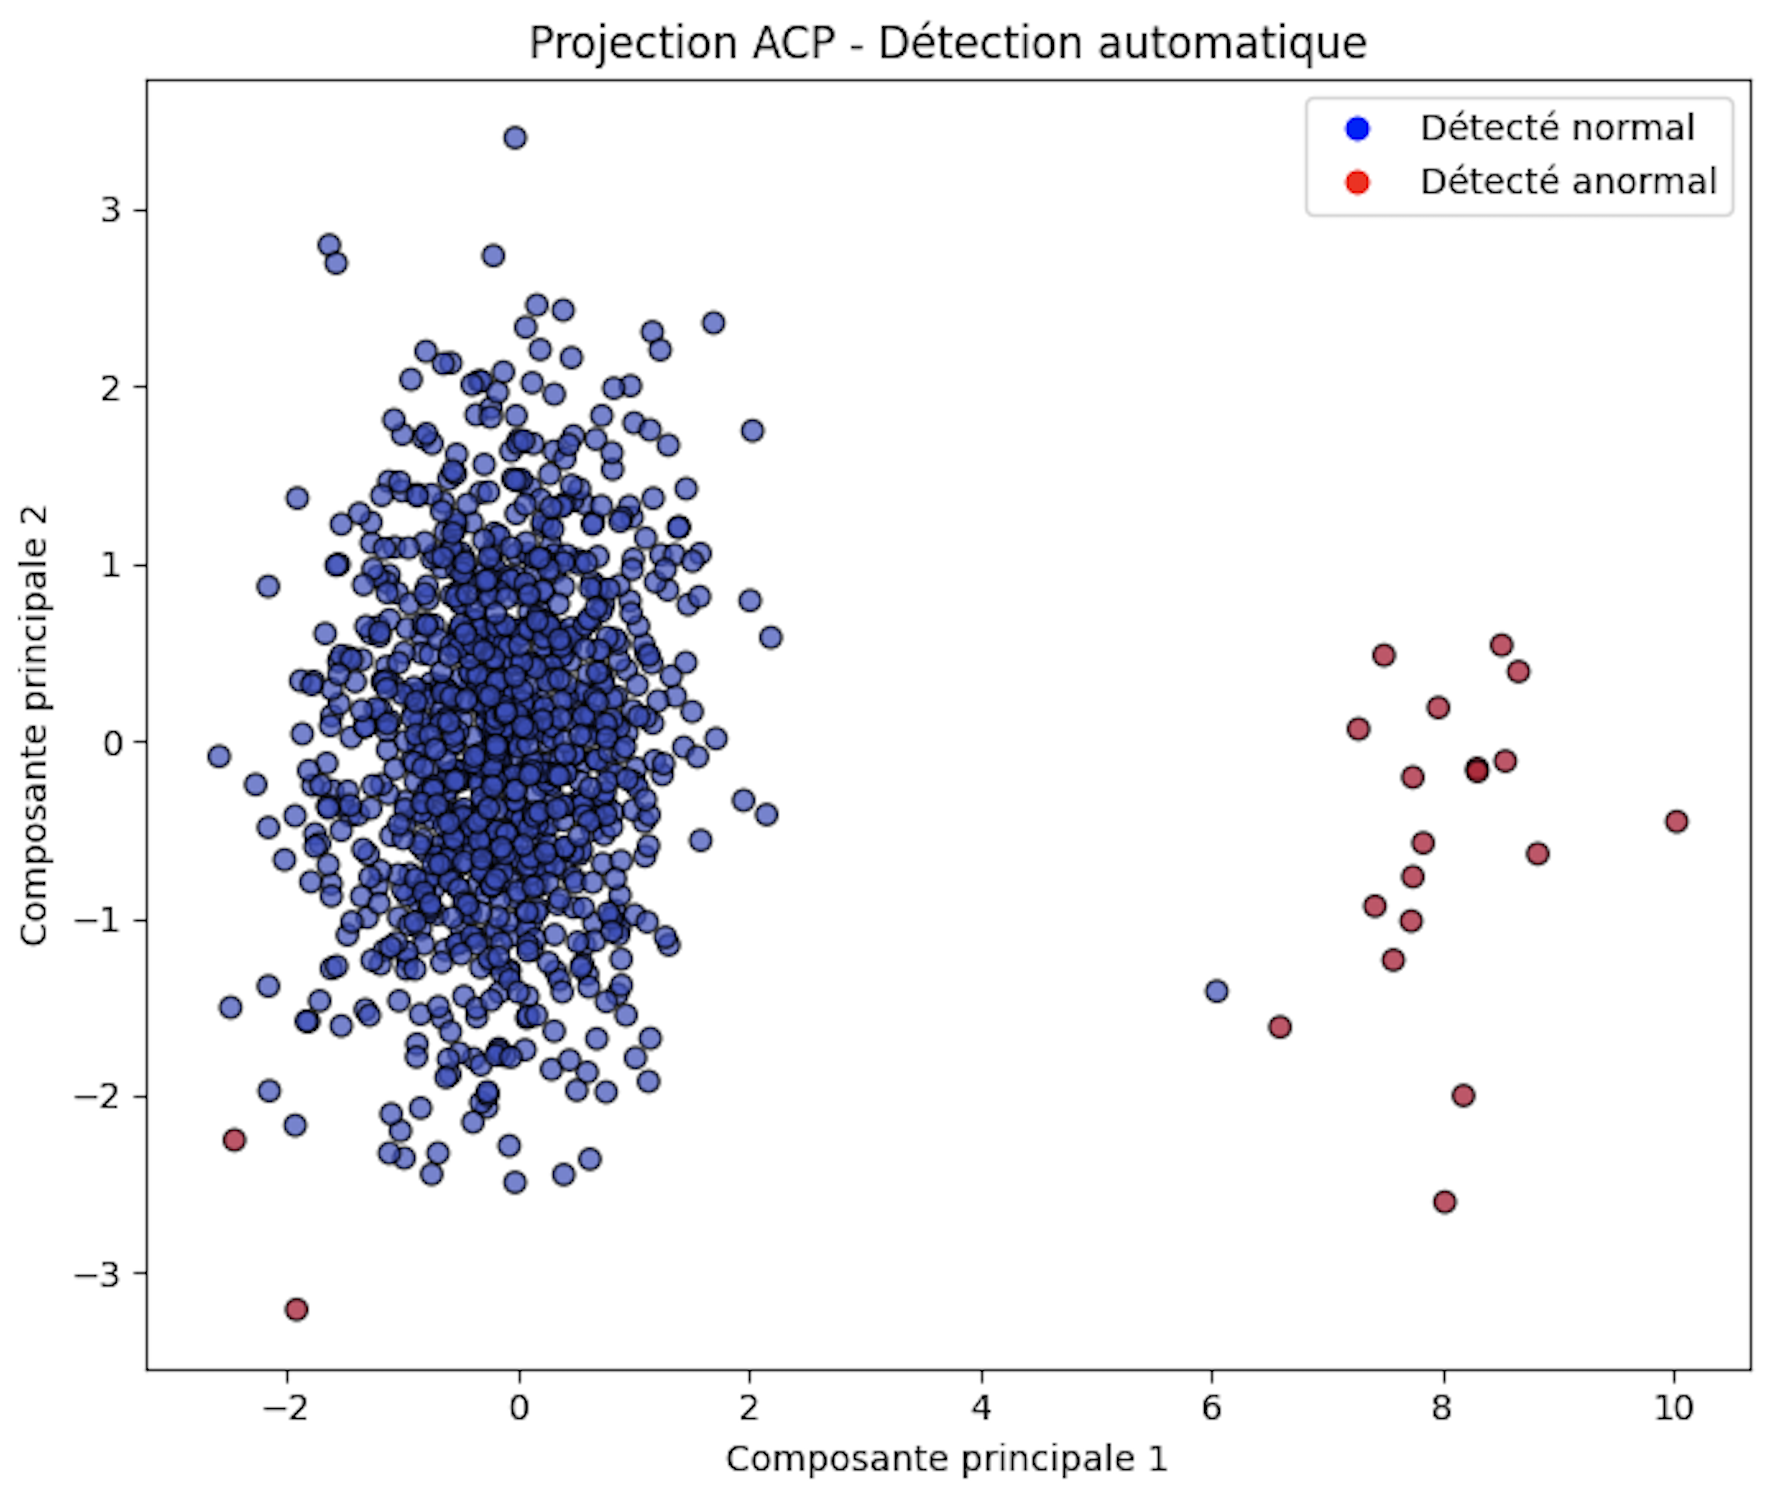
\includegraphics[width=0.8\textwidth]{projection_detection.png}
  \caption{Projection ACP - D\'etection par Isolation Forest : les anomalies d\'etect\'ees apparaissent isol\'ees.}
  \label{fig:detection}
\end{figure}

\subsection{Autres Applications Illustratives de l’ACP}

\subsubsection{Visualisation de la s\'eparation des classes}
L'ACP est souvent utilis\'ee pour explorer la s\'eparabilit\'e des classes dans les probl\`emes de classification supervis\'ee. En projetant les donn\'ees dans le plan form\'e par les deux premi\`eres composantes principales, on peut visualiser si les classes sont bien distinctes ou fortement entrem\^el\'ees.

\begin{figure}
  \centering
  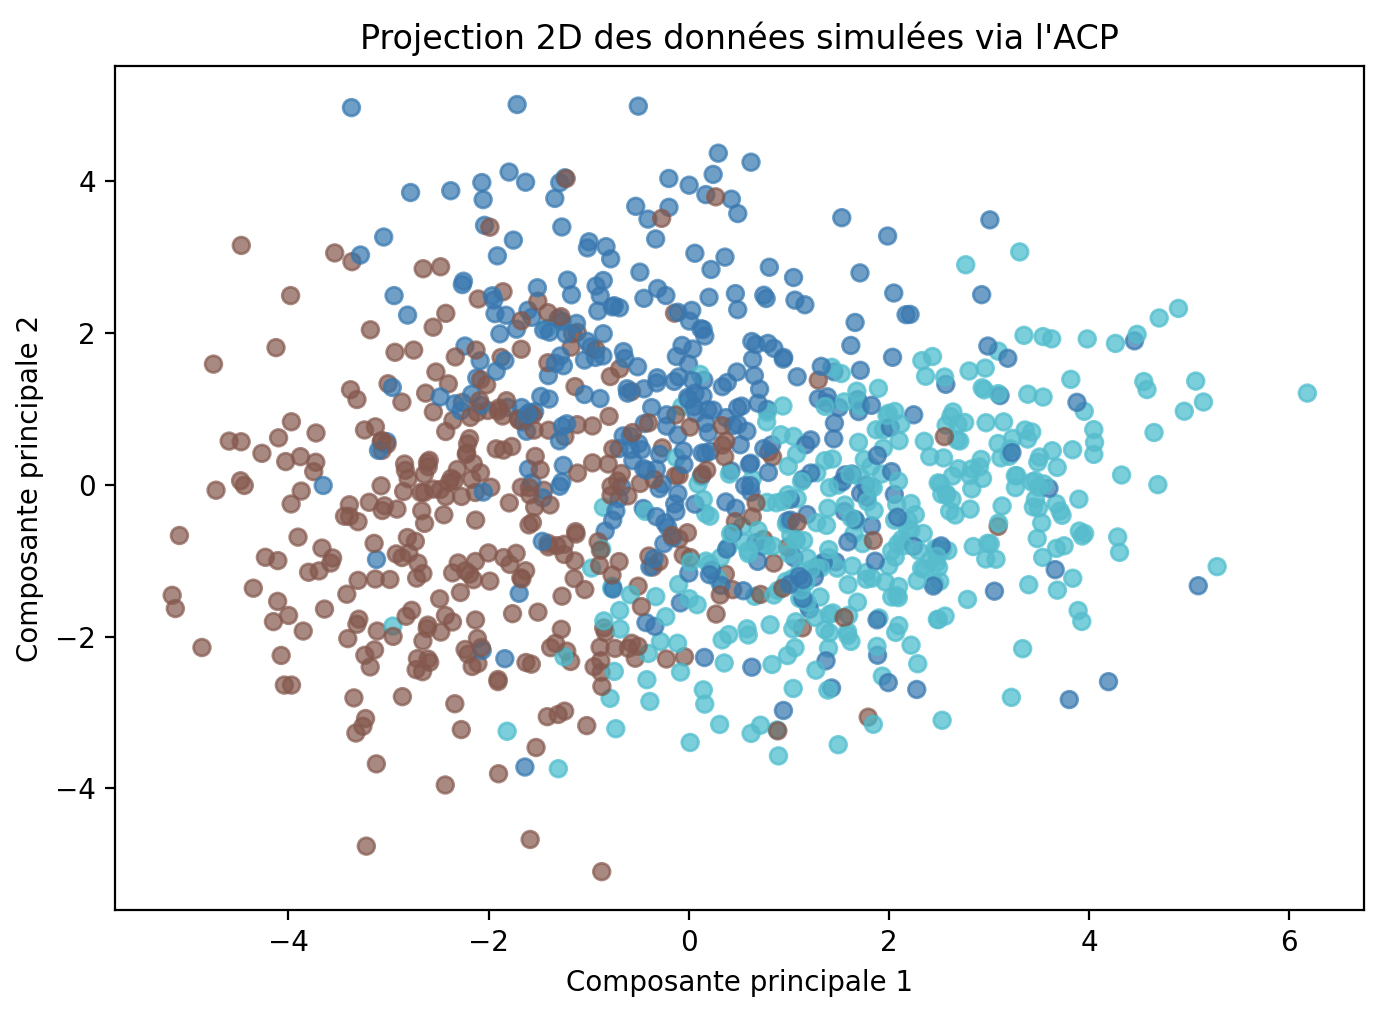
\includegraphics[width=0.8\textwidth]{separation_classes.png}   
  \caption{Projection ACP de donn\'ees \'etiquet\'ees montrant la s\'eparation entre deux classes.}
  \label{fig:separation_classes}
\end{figure}

\subsubsection{Analyse de la variance expliqu\'ee : Scree Plot}
Le \'el'ement cl\'e de l'ACP est la quantification de la variance captur\'ee par chaque composante. Le scree plot permet d'identifier combien de composantes suffisent \`a capturer l'information utile.

\begin{figure}[h!]
  \centering
  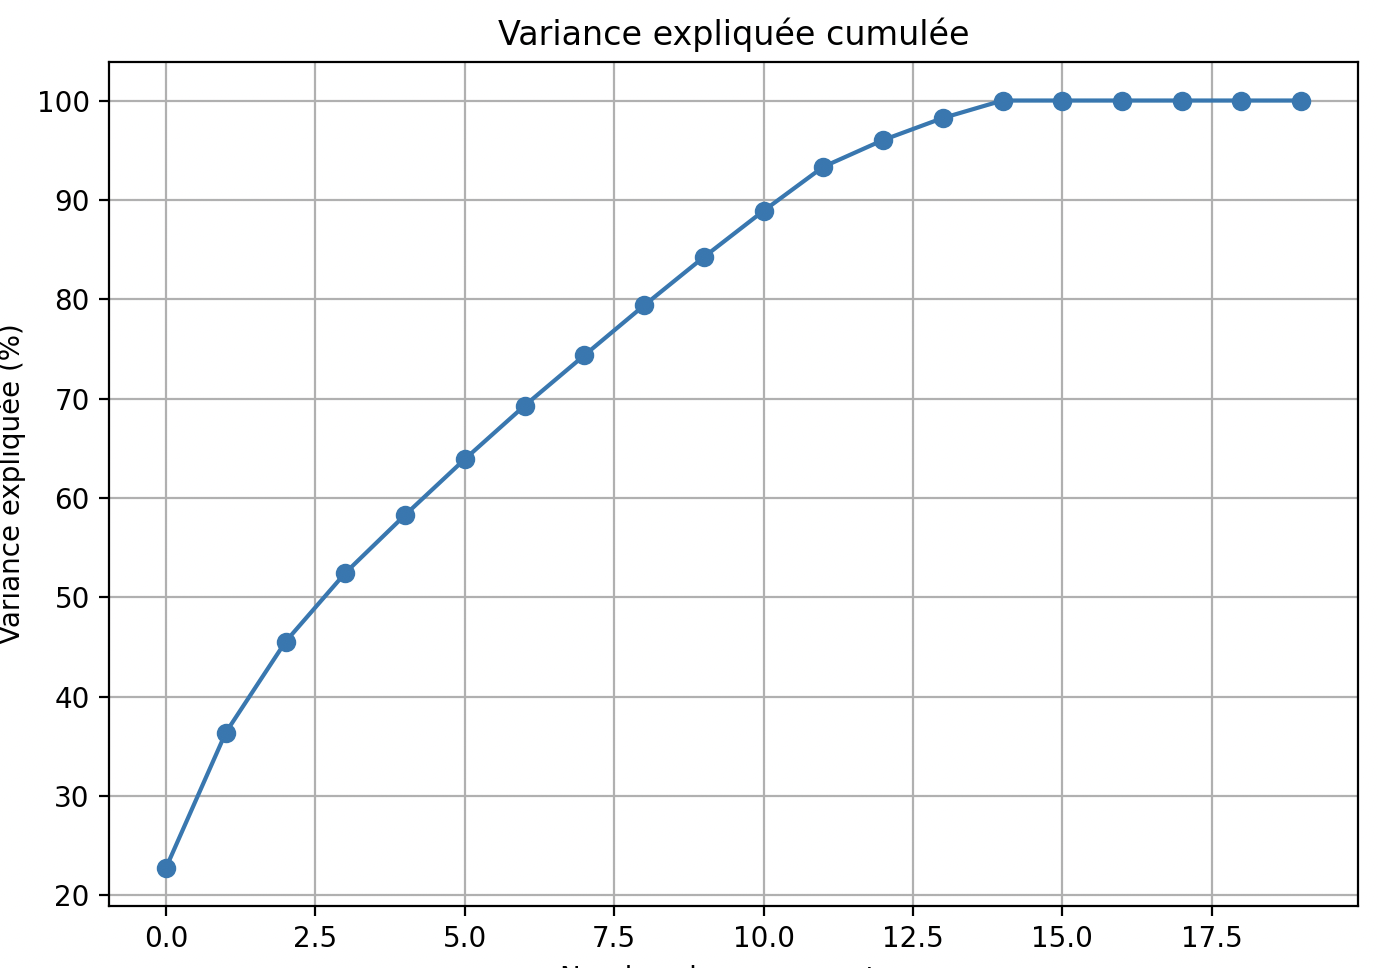
\includegraphics[width=0.7\textwidth]{scree_plot.png}   
  \caption{Scree plot montrant la variance expliqu\'ee par chaque composante principale.}
  \label{fig:scree_plot}
\end{figure}

\subsubsection{Filtrage de bruit : D\'ebruitage par ACP}
L'ACP peut \^etre utilis\'ee pour reconstruire un signal bruit\'e en conservant uniquement les composantes principales les plus significatives.

\begin{figure}[h!]
  \centering
  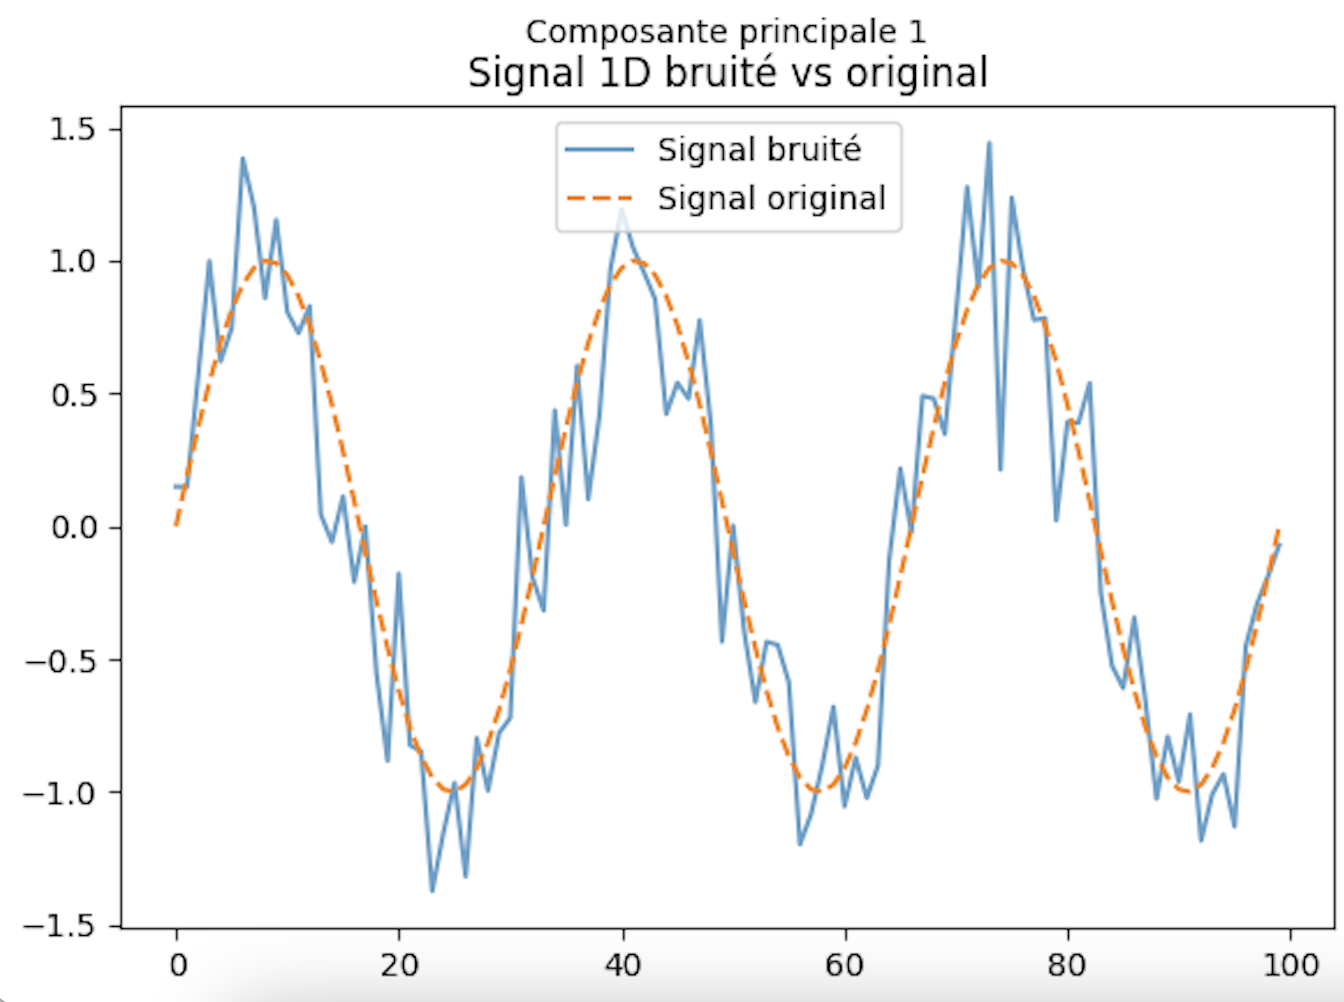
\includegraphics[width=0.45\textwidth]{signal_bruite.png}   
  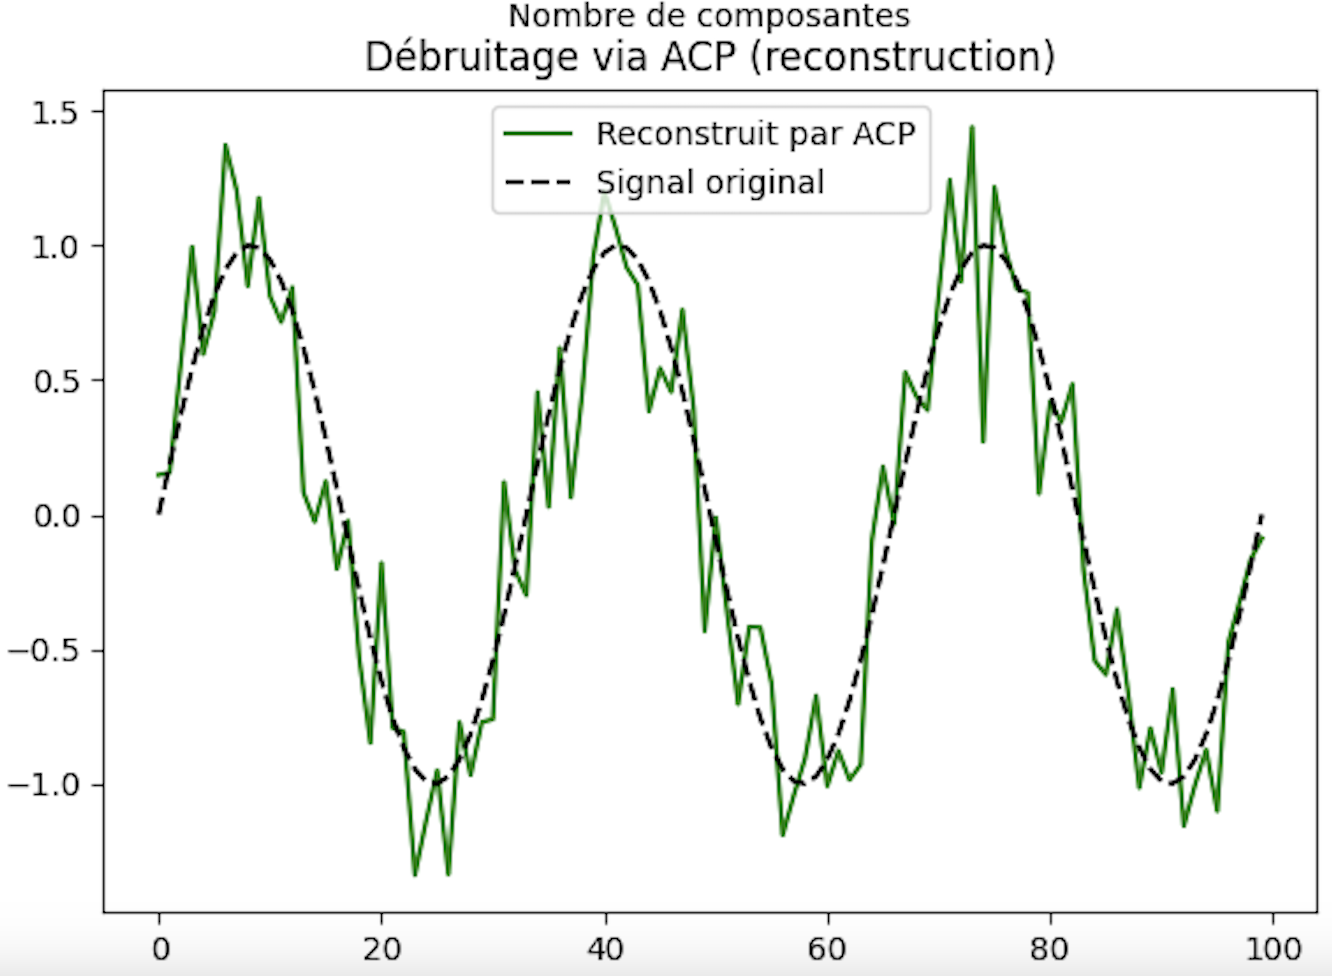
\includegraphics[width=0.45\textwidth]{signal_debruite.png}   
  \caption{\`A gauche : signal bruit\'e. \`A droite : signal reconstru\'it apr\`es d\'ebruitage par ACP.}
  \label{fig:debruitage}
\end{figure}

\subsection{Discussion}
L'utilisation de l'ACP permet de visualiser efficacement les regroupements naturels et les \textit{outliers}. Combin\'ee \`a un algorithme de d\'etection non supervis\'ee, elle facilite l'analyse des flux passagers en temps r\'eel sans surveillance humaine directe. Cette m\'ethode est \`a la fois rapide, explicable et g\'en\'eralisable \`a d'autres contextes de surveillance intelligente. Elle est \'egalement applicable \`a la classification, la compression, et le traitement du signal.

\subsection{Conclusion}
Ce chapitre a montr\'e comment l'ACP peut \^etre utilis\'ee comme une pr\'etraitement puissant pour la d\'etection d'anomalies dans des donn\'ees de haute dimension. Dans notre cas, elle permet une repr\'esentation 2D compr\'ehensible facilitant l'identification des comportements anormaux dans les environnements a\'eroportuaires, ainsi que d'autres usages vari\'es allant de la classification \`a la reconstruction de signaux.

\newpage
\chapter{Préliminaire}
\section{Préliminaires Mathématiques pour l'Analyse en Composantes Principales}

L'Analyse en Composantes Principales (ACP) repose sur plusieurs concepts mathématiques fondamentaux. Dans cette section, nous aborderons les notions essentielles qui préparent le terrain pour comprendre le processus de réduction de dimension à travers l'ACP.

\subsection{Statistiques de base et covariance}

La covariance entre deux variables \( X \) et \( Y \) mesure comment ces variables varient ensemble. Elle est définie par la formule suivante :

\[
\text{Cov}(X, Y) = \frac{1}{n} \sum_{i=1}^n (X_i - \bar{X})(Y_i - \bar{Y})
\]

où \( X_i \) et \( Y_i \) sont les observations des variables \( X \) et \( Y \), et \( \bar{X} \) et \( \bar{Y} \) sont leurs moyennes respectives.

Dans un espace multidimensionnel, la covariance peut être représentée par une **matrice de covariance**, où chaque élément \( C_{ij} \) représente la covariance entre les variables \( X_i \) et \( X_j \). Cette matrice est symétrique et joue un rôle clé dans l’ACP, car elle décrit les relations linéaires entre les différentes dimensions des données.

\begin{figure}[H]
    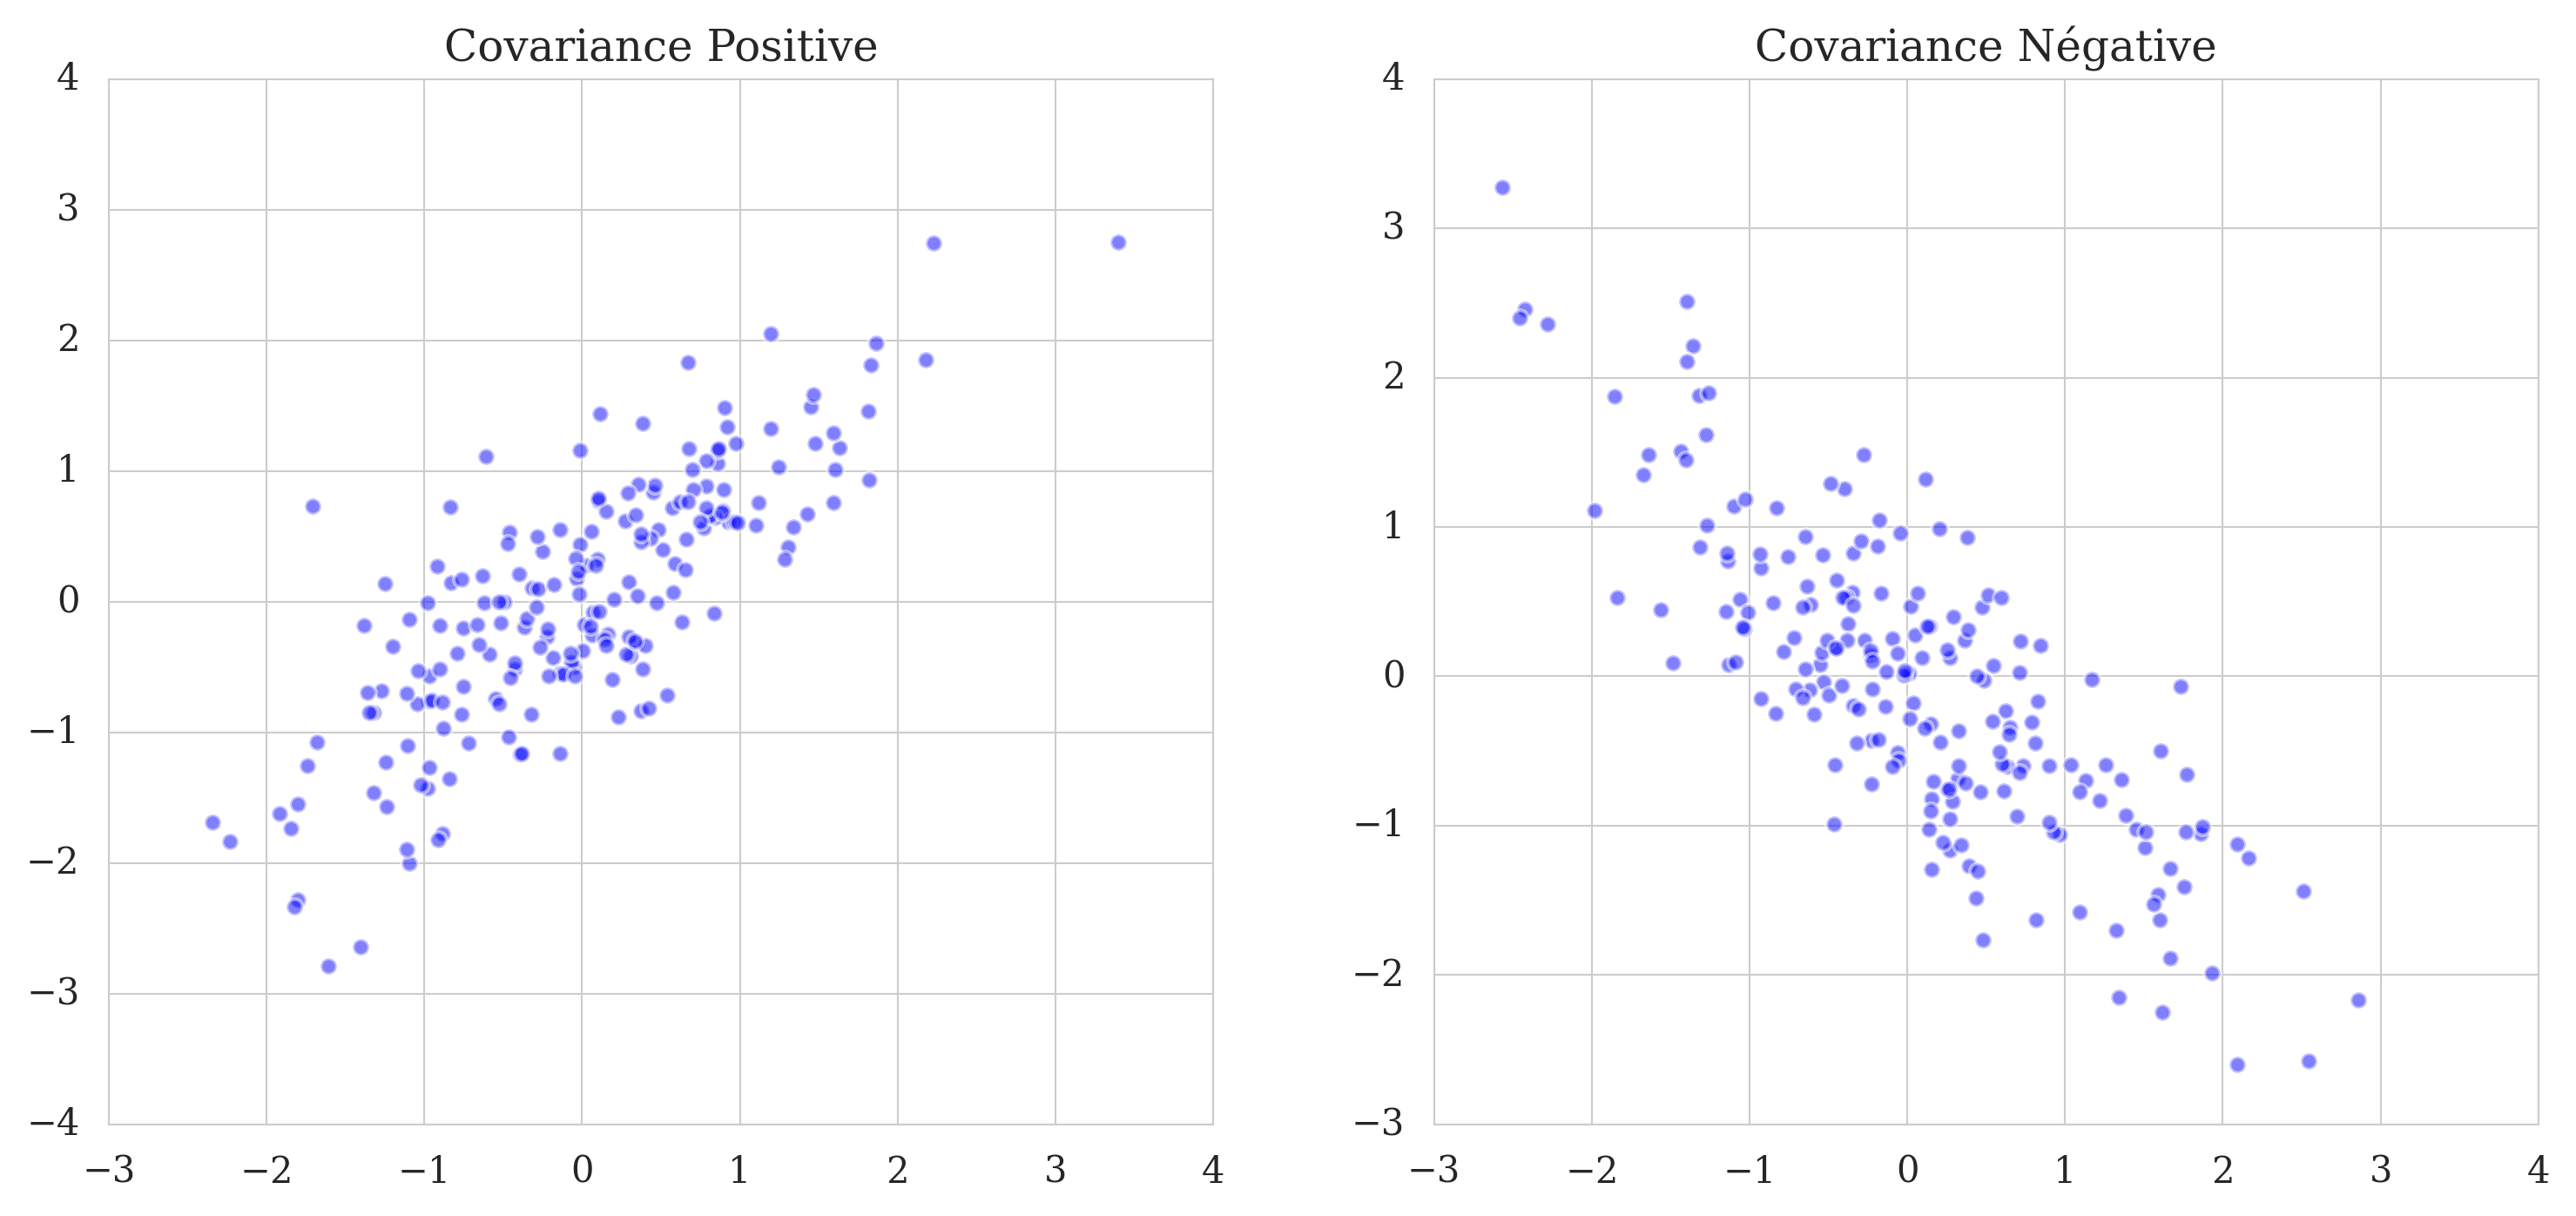
\includegraphics[width=1\textwidth]{covariance_illustration.png} 
    \caption{Illustration géométrique de la covariance. Lorsque la covariance est positive, les deux variables ont tendance à augmenter ensemble. Si la covariance est négative, elles varient en sens opposé.}
    \label{fig:covariance}
\end{figure}

La figure \ref{fig:covariance} montre deux ensembles de points où la covariance entre les deux variables est positive (à gauche) et négative (à droite).

\subsection{Diagonalisation et valeurs propres}

La diagonalisation d'une matrice de covariance est au cœur de l'ACP. En trouvant les **valeurs propres** et **vecteurs propres** de cette matrice, on peut identifier les directions dans lesquelles les données varient le plus. Chaque valeur propre représente l'importance d'une direction, et le vecteur propre associé représente l'orientation de cette direction dans l'espace.

\begin{figure}[H]
    \centering
    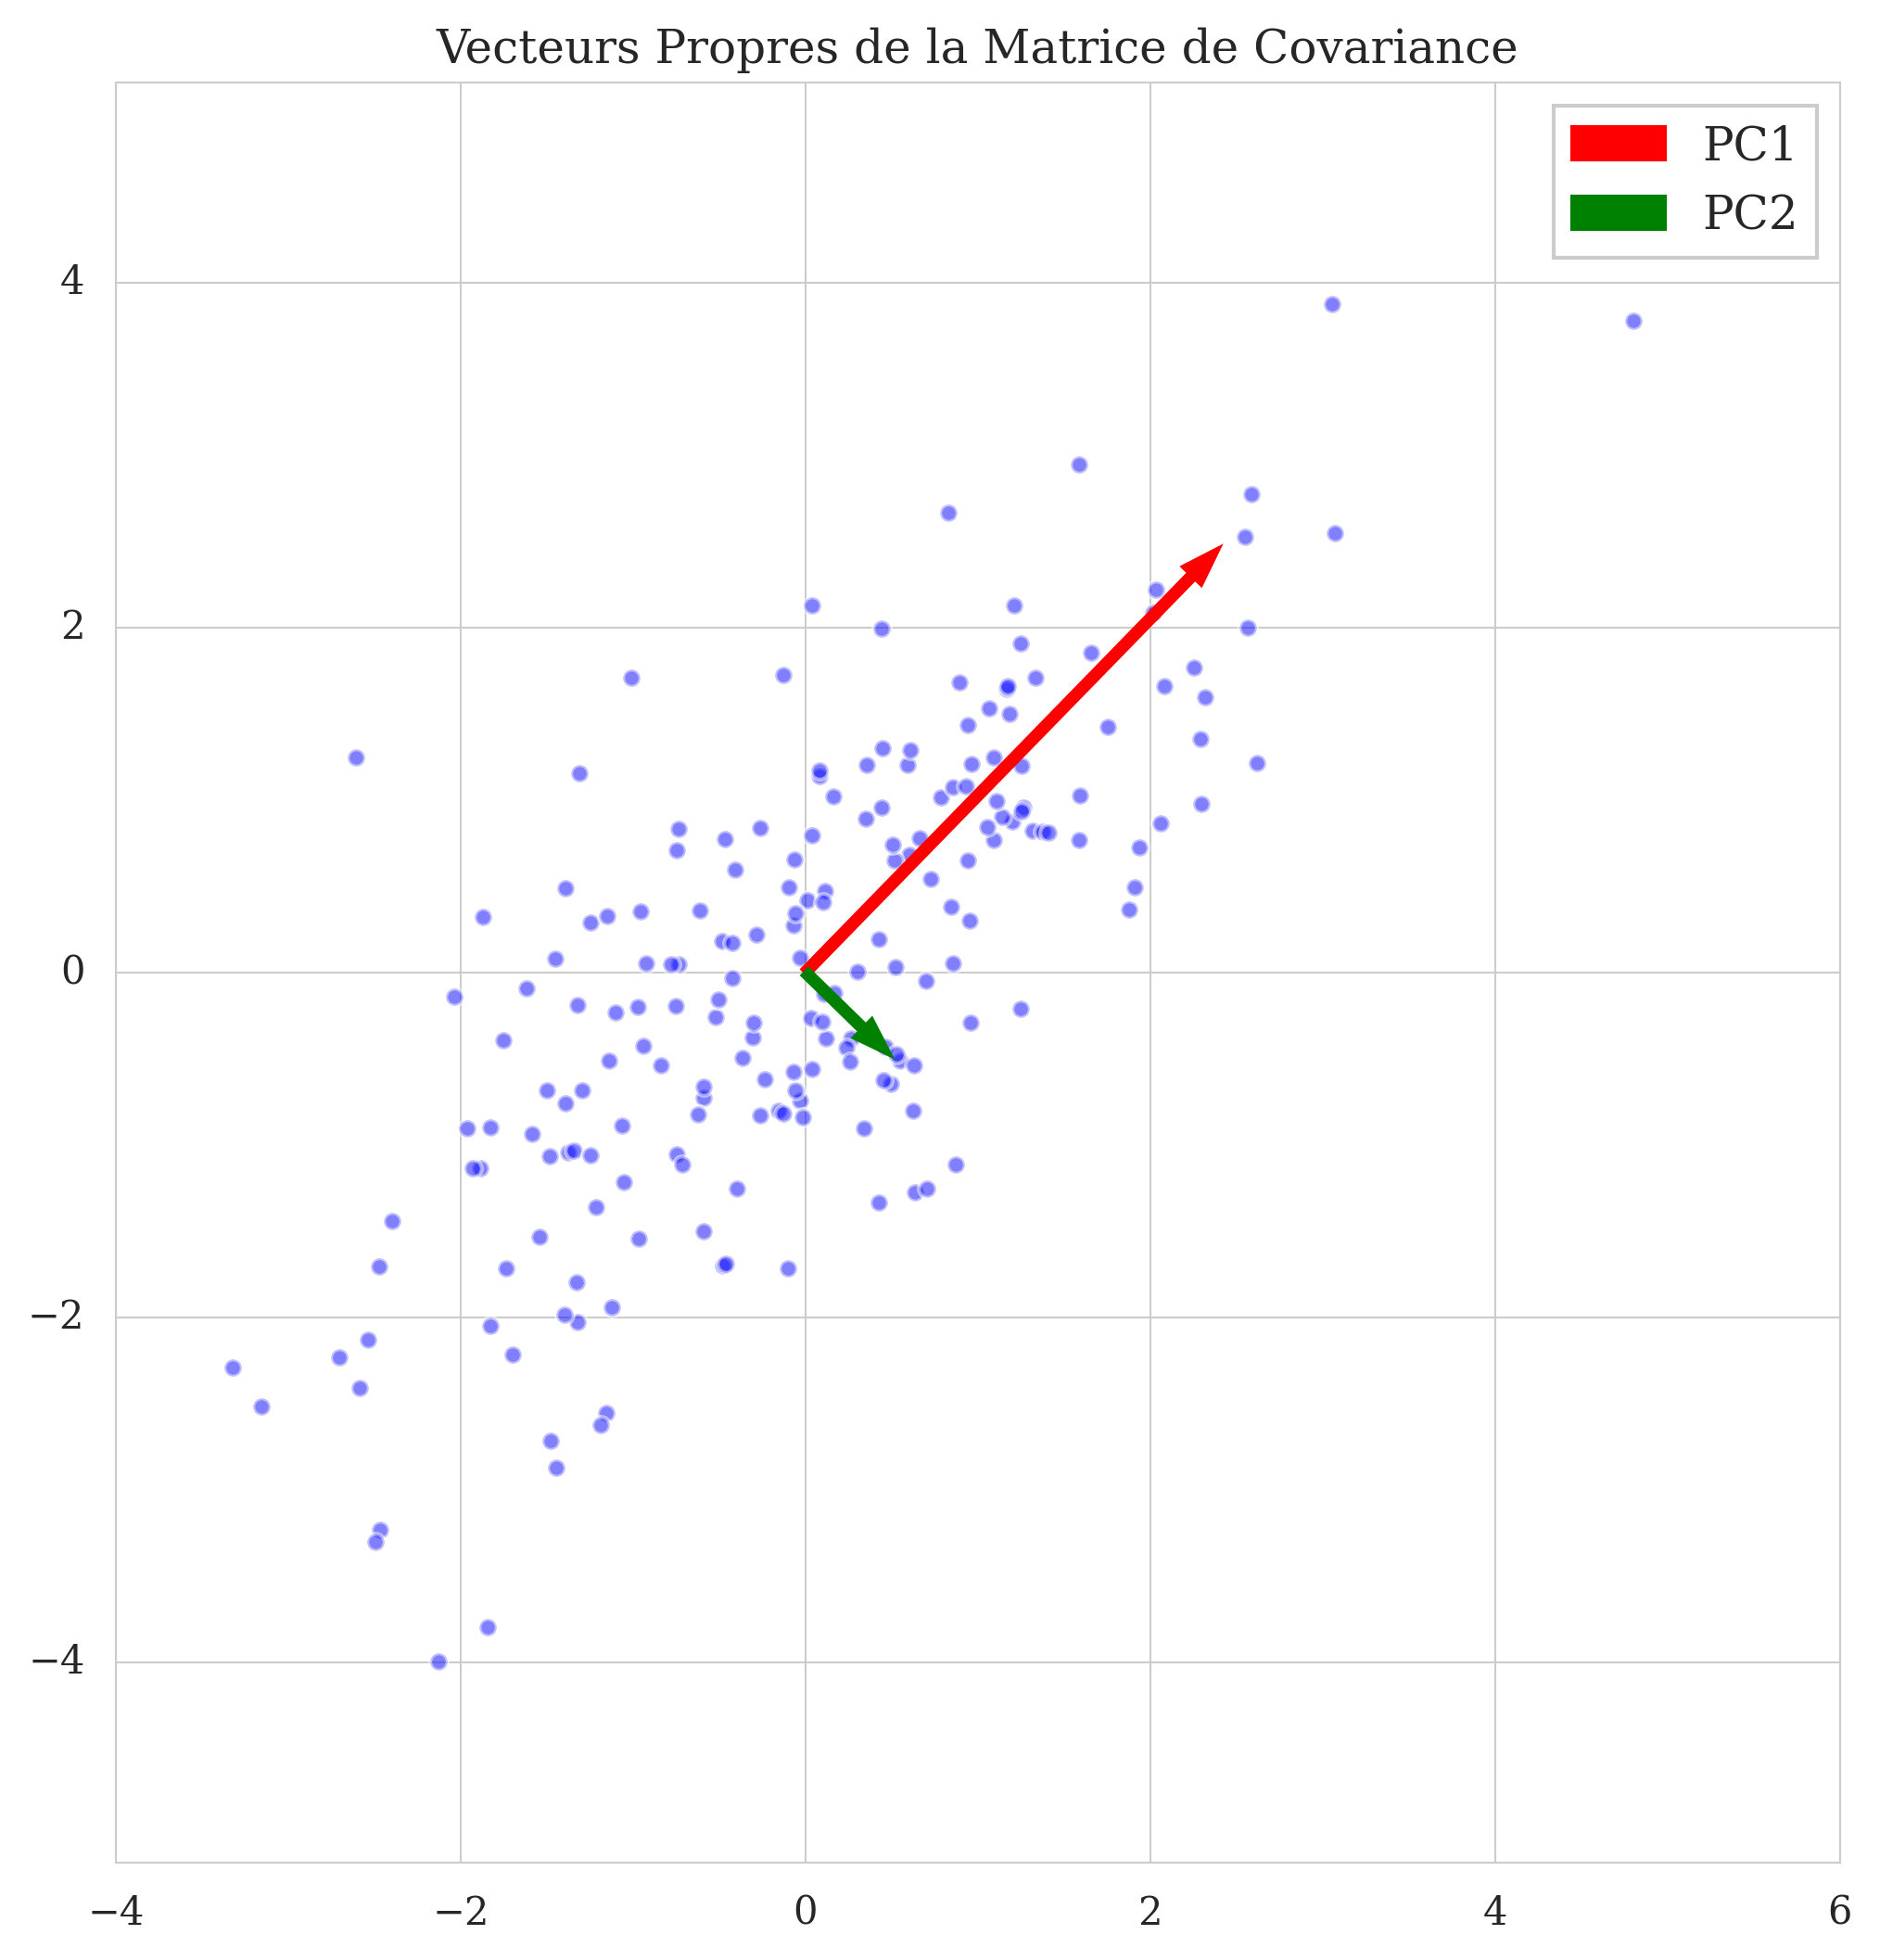
\includegraphics[width=0.9\textwidth]{eigenvec.png}
    \caption{Représentation des valeurs propres et des vecteurs propres dans l'espace des données. Les vecteurs propres indiquent les directions de la variance maximale.}
    \label{fig:valeurs_propres}
\end{figure}

La figure \ref{fig:valeurs_propres} montre comment les vecteurs propres sont les directions principales dans lesquelles les données sont les plus dispersées. Les valeurs propres associées à ces vecteurs indiquent l’importance de chaque direction.


\subsection{Décomposition en valeurs singulières}

La décomposition en valeurs singulières (SVD) factorise toute matrice réelle $X$ en composantes orthogonales et valeurs singulières.

\paragraph*{Définition (SVD)}%
Pour toute matrice $X\in\mathbb{R}^{m\times n}$, il existe des matrices orthogonales 
$U\in\mathbb{R}^{m\times m}$ et $V\in\mathbb{R}^{n\times n}$ ainsi qu’une matrice diagonale 
$\Sigma\in\mathbb{R}^{m\times n}$,  
\[
\Sigma = \operatorname{diag}(\sigma_1,\ldots,\sigma_r),
\quad \sigma_1\ge \sigma_2\ge\cdots\ge \sigma_r\ge 0,
\]
telles que
\[
X = U\,\Sigma\,V^{\top}.
\]

\paragraph*{Corollaire (calcul de $X^{\top}X$)}%
On en déduit immédiatement que
\[
X^{\top}X = V\,\Sigma^{2}\,V^{\top}
= V\,\operatorname{diag}(\sigma_1^{2},\ldots,\sigma_r^{2})\,V^{\top},
\]
ce qui fournit directement les valeurs propres de $X^{\top}X$ (utile pour l’ACP).




\subsection{Centrage et normalisation des données}

Avant d'appliquer l'ACP, il est crucial de centrer les données. Cela signifie soustraire la moyenne de chaque dimension pour que les données aient une moyenne nulle. Ce centrage est nécessaire pour éviter que les composantes principales ne soient biaisées par des différences dans les échelles des dimensions.

\begin{figure}[H]
    \centering
    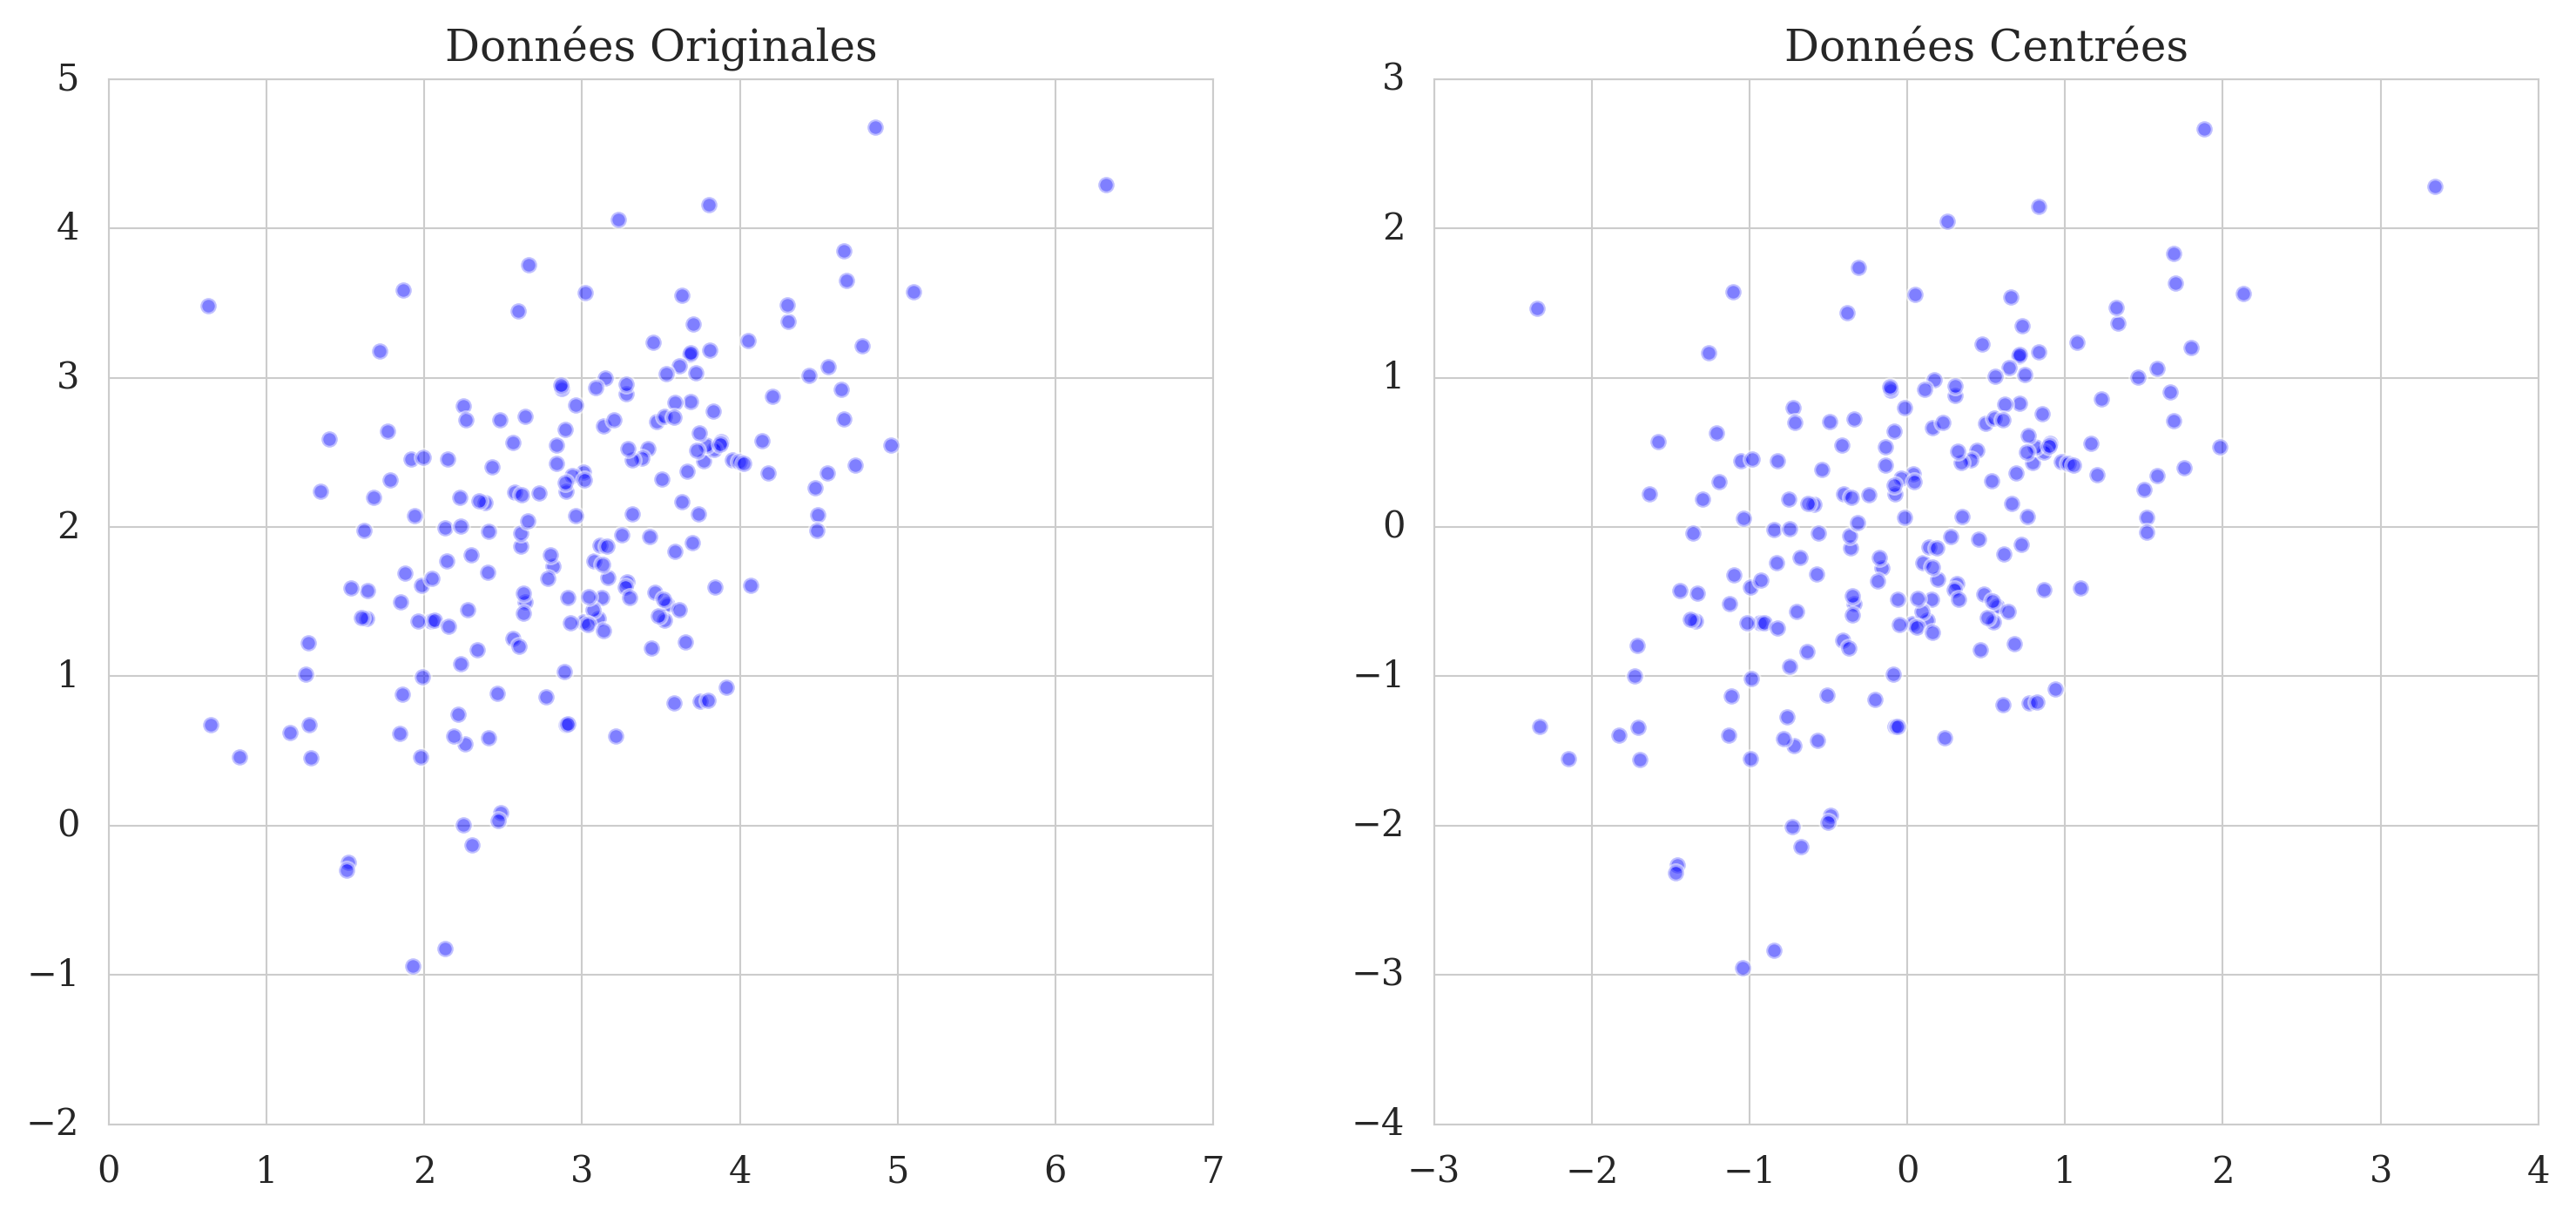
\includegraphics[width=1.1\textwidth]{centrage_normalisation.png}
    \caption{Illustration du centrage des données. Chaque dimension est ajustée de manière à avoir une moyenne nulle.}
    \label{fig:centrage}
\end{figure}

\subsection{Extraction des valeurs propres et vecteurs propres}
Pour extraire le spectre de la matrice de covariance \(\Sigma\), plusieurs méthodes numériques peuvent être utilisées. Voici quelques approches classiques et leur algorithme détaillé :

\begin{enumerate}
    \item \textbf{Méthode de la puissance (Power Iteration) :}
    \begin{enumerate}
        \item Choisir un vecteur initial aléatoire non nul \(v^{(0)}\).
        \item Pour \(k=1,2,\ldots\) jusqu'à convergence, calculer
        \[
        v^{(k)} = \frac{\Sigma\, v^{(k-1)}}{\|\Sigma\, v^{(k-1)}\|}.
        \]
        \item Lorsque \(\|v^{(k)} - v^{(k-1)}\| < \epsilon\), estimer la plus grande valeur propre par
        \[
        \lambda_{\max} \approx {v^{(k)}}^\top \Sigma\, v^{(k)}.
        \]
    \end{enumerate}
    \item \textbf{Déflation :}  
    Une fois obtenue la plus grande valeur propre \(\lambda_1\) et son vecteur \(v_1\), soustraire leur contribution :
    \[
    \Sigma^{(1)} = \Sigma - \lambda_1\, v_1\, v_1^\top.
    \]
    Puis répéter la méthode de la puissance sur \(\Sigma^{(1)}\) afin d'extraire les valeurs et vecteurs suivants.
    
    \item \textbf{Algorithme QR :}
    \begin{enumerate}
        \item Initialiser une matrice orthonormale \(Q^{(0)}\) de dimension \(p\times p\).
        \item Pour \(k=1,2,\ldots\) :
        \begin{enumerate}
            \item Décomposer la matrice actuelle :
            \[
            A^{(k-1)} = Q^{(k)}\, R^{(k)},
            \]
            où \(A^{(0)} = \Sigma\).
            \item Mettre à jour :
            \[
            A^{(k)} = R^{(k)}\, Q^{(k)}.
            \]
        \end{enumerate}
        \item Lorsque \(A^{(k)}\) converge vers une matrice presque diagonale, les éléments diagonaux de \(A^{(k)}\) approchent les valeurs propres de \(\Sigma\) et les colonnes de \(Q^{(k)}\) fournissent les vecteurs propres correspondants.
    \end{enumerate}
    
    \item \textbf{Méthode de Jacobi (pour matrices symétriques) :}
    \begin{enumerate}
        \item Choisir un couple d'indices \((i,j)\) avec \(i\neq j\) tel que l'élément hors-diagonale \(\Sigma_{ij}\) soit maximal.
        \item Calculer l'angle de rotation \(\theta\) qui annule cet élément, puis former la matrice de rotation \(J(i,j,\theta)\).
        \item Mettre à jour la matrice par :
        \[
        \Sigma \leftarrow J^\top\, \Sigma\, J.
        \]
        \item Répéter ces itérations jusqu'à ce que tous les éléments hors-diagonaux soient inférieurs à un seuil fixé.
        \item La matrice finale sera approximativement diagonale et ses éléments diagonaux représenteront les valeurs propres, les rotations accumulées donnant les vecteurs propres.
    \end{enumerate}
\end{enumerate}

\begin{figure}[H]
\fbox{\parbox{\textwidth}{
\textbf{Algorithme :} Extraction des valeurs propres et vecteurs propres via Power Iteration, Déflation, et QR
\begin{enumerate}
    \item \textbf{Power Iteration pour la plus grande valeur propre} :
    \begin{enumerate}
        \item Choisir \(v^{(0)}\) arbitraire (non nul).
        \item Pour \(k=1,2,\ldots\), calculer
        \[
        v^{(k)} = \frac{\Sigma\, v^{(k-1)}}{\|\Sigma\, v^{(k-1)}\|}.
        \]
        \item Convergence lorsque \(\|v^{(k)} - v^{(k-1)}\| < \epsilon\); estimer
        \[
        \lambda_1 \approx {v^{(k)}}^\top \Sigma\, v^{(k)}.
        \]
    \end{enumerate}
    \item \textbf{Déflation} pour extraire les composantes suivantes :
    \begin{enumerate}
        \item Calculer \(\Sigma^{(1)} = \Sigma - \lambda_1\, v^{(k)}{v^{(k)}}^\top\).
        \item Répéter la méthode de la puissance sur \(\Sigma^{(1)}\) pour obtenir \(\lambda_2\) et \(v_2\), etc.
    \end{enumerate}
    \item \textbf{Méthode QR} :
    \begin{enumerate}
        \item Initialiser \(A^{(0)} = \Sigma\) et une matrice orthonormale \(Q^{(0)}\).
        \item Pour \(k=1,2,\ldots\) :
        \begin{enumerate}
            \item Calculer la décomposition \(A^{(k-1)} = Q^{(k)} R^{(k)}\).
            \item Mettre à jour \(A^{(k)} = R^{(k)} Q^{(k)}\).
        \end{enumerate}
        \item Lorsque \(A^{(k)}\) devient presque diagonale, les diagonales approchent \(\lambda_i\) et les colonnes de \(Q^{(k)}\) approchent \(w_i\).
    \end{enumerate}
\end{enumerate}
}}
\caption{Extraction des valeurs propres et vecteurs propres (Power Iteration, Déflation, et QR)}
\label{alg:eigd}
\end{figure}

---

**Résumé des concepts clés :**
- **Covariance** : Comprendre comment les variables sont corrélées entre elles.
- **Transformation linéaire** : Réduire la dépendance entre les variables.
- **Diagonalisation** : Identifier les directions principales dans les données via les vecteurs propres.
- **SVD** : Utiliser la décomposition pour réaliser une réduction dimensionnelle.
- **Centrage des données** : Préparer les données avant l'ACP.

---

Cela couvre les concepts nécessaires pour préparer le terrain pour l'ACP dans ton projet. Si tu as besoin de plus de détails ou de modifications, n’hésite pas à me le faire savoir !

\chapter{Analyse en Composantes Principales (PCA)}

\section{Formulation mathématique}

Soit \( X \in \mathbb{R}^{n \times p} \) une matrice de données centrée (chaque colonne a une moyenne nulle). On cherche à projeter les données sur une direction \( w \in \mathbb{R}^p \) de manière à maximiser la variance des projections.

\subsection{Problème d'optimisation fondamental}

L’objectif de la PCA peut être formulé comme un problème d’optimisation quadratique sous contrainte :

\begin{equation}
\begin{aligned}
\max_{w \in \mathbb{R}^p} \quad & \text{Var}(X w) = w^\top \Sigma w \\
\text{sous la contrainte} \quad & \|w\|^2 = 1
\end{aligned}
\end{equation}

où \( \Sigma = \frac{1}{n-1} X^\top X \) est la matrice de covariance des données.

Ce problème est un cas classique de maximisation quadratique sous contrainte quadratique. Sa solution est donnée par le théorème des multiplicateurs de Lagrange : le vecteur \( w \) qui maximise cette expression est le **vecteur propre associé à la plus grande valeur propre de \( \Sigma \)**.

\subsection{Dérivation complète de l'ACP}

La recherche successive des composantes principales peut être formulée comme une série de problèmes d'optimisation. Pour la k-ième composante, nous cherchons :

\begin{equation}
\begin{aligned}
\max_{w_k \in \mathbb{R}^p} \quad & w_k^\top \Sigma w_k \\
\text{sous les contraintes} \quad & \|w_k\|^2 = 1 \\
& w_k^\top w_j = 0, \quad \forall j < k
\end{aligned}
\end{equation}

  
\subsubsection*{Rappel sur la méthode des multiplicateurs de Lagrange}
Soit un problème d'optimisation sous contrainte classique :
\begin{equation}
    \begin{aligned}
        & \max_{x \in \mathbb{R}^n} && f(x) \\
        & \text{sous la contrainte} && g(x) = 0,
    \end{aligned}
\end{equation}
dans lequel $f : \mathbb{R}^n \to \mathbb{R}$ et $g : \mathbb{R}^n \to \mathbb{R}$ sont deux fonctions suffisamment régulières. 

L'idée clé de la méthode est d'introduire un multiplicateur de Lagrange $\lambda \in \mathbb{R}$ pour incorporer la contrainte au problème non contraint :
\begin{equation}
    \mathcal{L}(x,\lambda) = f(x) - \lambda\, g(x).
\end{equation}

Les conditions d'optimalité (nécéssaires sous hypothèse de régularité) se formalisent par :
\begin{equation}
    \begin{cases}
        \nabla_x \mathcal{L}(x,\lambda) = 0,  \\
        g(x) = 0.
    \end{cases}
\end{equation}

Concrètement, la première équation dit que, au point optimal, le gradient de la fonction objectif doit être colinéaire au gradient de la contrainte ; le multiplicateur $\lambda$ fixe le facteur de proportionnalité.

  
\subsubsection{Application au calcul de la première composante principale}
Dans le cadre de l'analyse en composantes principales (ACP), on cherche un vecteur unitaire $w$ qui maximise la variance projetée :
\begin{equation}
    \max_{w \in \mathbb{R}^d} \; w^\top \Sigma \; w
    \quad\text{sous la contrainte}\quad
    w^\top w = 1,
\end{equation}
où $\Sigma$ est la matrice de covariance centrée des données.  
On pose donc :
\begin{equation}
    f(w) = w^\top \Sigma w, 
    \qquad g(w) = w^\top w - 1.
\end{equation}
et l'on construit le Lagrangien :
\begin{equation}
    \mathcal{L}(w,\lambda) 
    = f(w) - \lambda\,g(w)
    = w^\top \Sigma w 
      - \lambda\,(w^\top w - 1).
\end{equation}

Les conditions d'optimalité s'écrivent alors :
\begin{equation}
    \nabla_w \mathcal{L}(w,\lambda) = 0
    \quad\Longrightarrow\quad
    2\,\Sigma w - 2\,\lambda w = 0
    \quad\Longleftrightarrow\quad
    \Sigma w = \lambda\,w.
\end{equation}
On reconnait l'équation aux valeurs propres de la matrice $\Sigma$, avec $\lambda" class="math inline"> la valeur propre associée au vecteur propre $w". 

Concluons que pour maximiser la variance projetée, on choisit $w" class="math inline"> égal à l'autovecteur associé à la plus grande valeur propre de $\Sigma$.

  
\textbf{Remarque.}  
La contrainte $w^\top w = 1$ garantit l'unicité (à signe près) de la solution et évite la possibilité de faire croître indéfiniment $w$ pour augmenter $f(w)$ sans limite.

\subsection{Propriétés importantes}

\begin{enumerate}
    \item \textbf{Orthogonalité} : Les vecteurs propres $w_1, \ldots, w_p$ forment une base orthonormée de $\mathbb{R}^p$.
    
    \item \textbf{Variance expliquée} : La variance totale est conservée et égale à la somme des valeurs propres :
    \[\sum_{i=1}^p \lambda_i = \text{tr}(\Sigma) = \sum_{j=1}^p \text{Var}(X_j)\]
    
    \item \textbf{Proportion de variance} : La proportion de variance expliquée par la k-ième composante est :
    \[\frac{\lambda_k}{\sum_{i=1}^p \lambda_i}\]
\end{enumerate}
\begin{figure}[H]
\fbox{\parbox{\textwidth}{
\textbf{Algorithme :} Calcul des composantes principales
\begin{enumerate}
    \item Centrer les données : $X_{c} = X - \bar{X}$
    \item Calculer la matrice de covariance : $\Sigma = \frac{1}{n-1}X_{c}^\top X_{c}$
    \item Calculer les valeurs propres $\lambda_i$ et vecteurs propres $w_i$ de $\Sigma$
    \item Trier les vecteurs propres par valeurs propres décroissantes
    \item Projeter les données : $Y = X_{c}W$ où $W = [w_1 \cdots w_k]$
\end{enumerate}
}}
\caption{Calcul des composantes principales}
\label{alg:pca}
\end{figure}

\subsection{Choix du nombre de composantes}

Pour sélectionner le nombre optimal de composantes, plusieurs critères peuvent être utilisés :
\begin{itemize}
    \item \textbf{Critère du coude} : Observer le point d'inflexion dans le scree plot.
    \item \textbf{Variance expliquée cumulée} : 
    Calculer la variance expliquée par les k premières composantes via la formule :
    \[
    \text{Ratio}_k = \frac{\sum_{i=1}^k \lambda_i}{\sum_{i=1}^{p} \lambda_i}
    \]
    Par exemple, si les valeurs propres sont $\lambda_1=3$, $\lambda_2=2$, $\lambda_3=1$, et $\lambda_4=0.5$, la variance totale vaut $6.5$. Pour $k=3$, on a :
    \[
    \text{Ratio}_3 = \frac{3+2+1}{6.5}\approx 0.92 \quad (92\  
    \]
    On retiendra alors $k=3$ si l'objectif est d'expliquer au moins 80 à 90\  
    
    \item \textbf{Critère de Kaiser} : 
    Lorsqu'on travaille avec des données standardisées (chaque variable ayant une variance de 1), la matrice de covariance possède une diagonale égale à 1. Ainsi, chaque valeur propre représente la variance expliquée par une composante et le critère recommande de retenir celles ayant $\lambda_i > 1$, c'est-à-dire une variance supérieure à celle d'une variable initiale.
    Par exemple, si les valeurs propres d'un jeu de données standardisé sont $\lambda_1=2.5$, $\lambda_2=1.2$, $\lambda_3=0.7$, et $\lambda_4=0.6$, seules les deux premières composantes seront retenues car elles satisfont $\lambda_i > 1$.
\end{itemize}

\subsection{Interprétation géométrique}

L'ACP peut être interprétée comme une rotation rigide de l'espace des données qui :
\begin{itemize}
    \item Aligne le premier axe avec la direction de variance maximale
    \item Aligne les axes suivants orthogonalement, maximisant la variance résiduelle
    \item Préserve les distances entre les points
\end{itemize}

\begin{figure}[H]
    \centering
    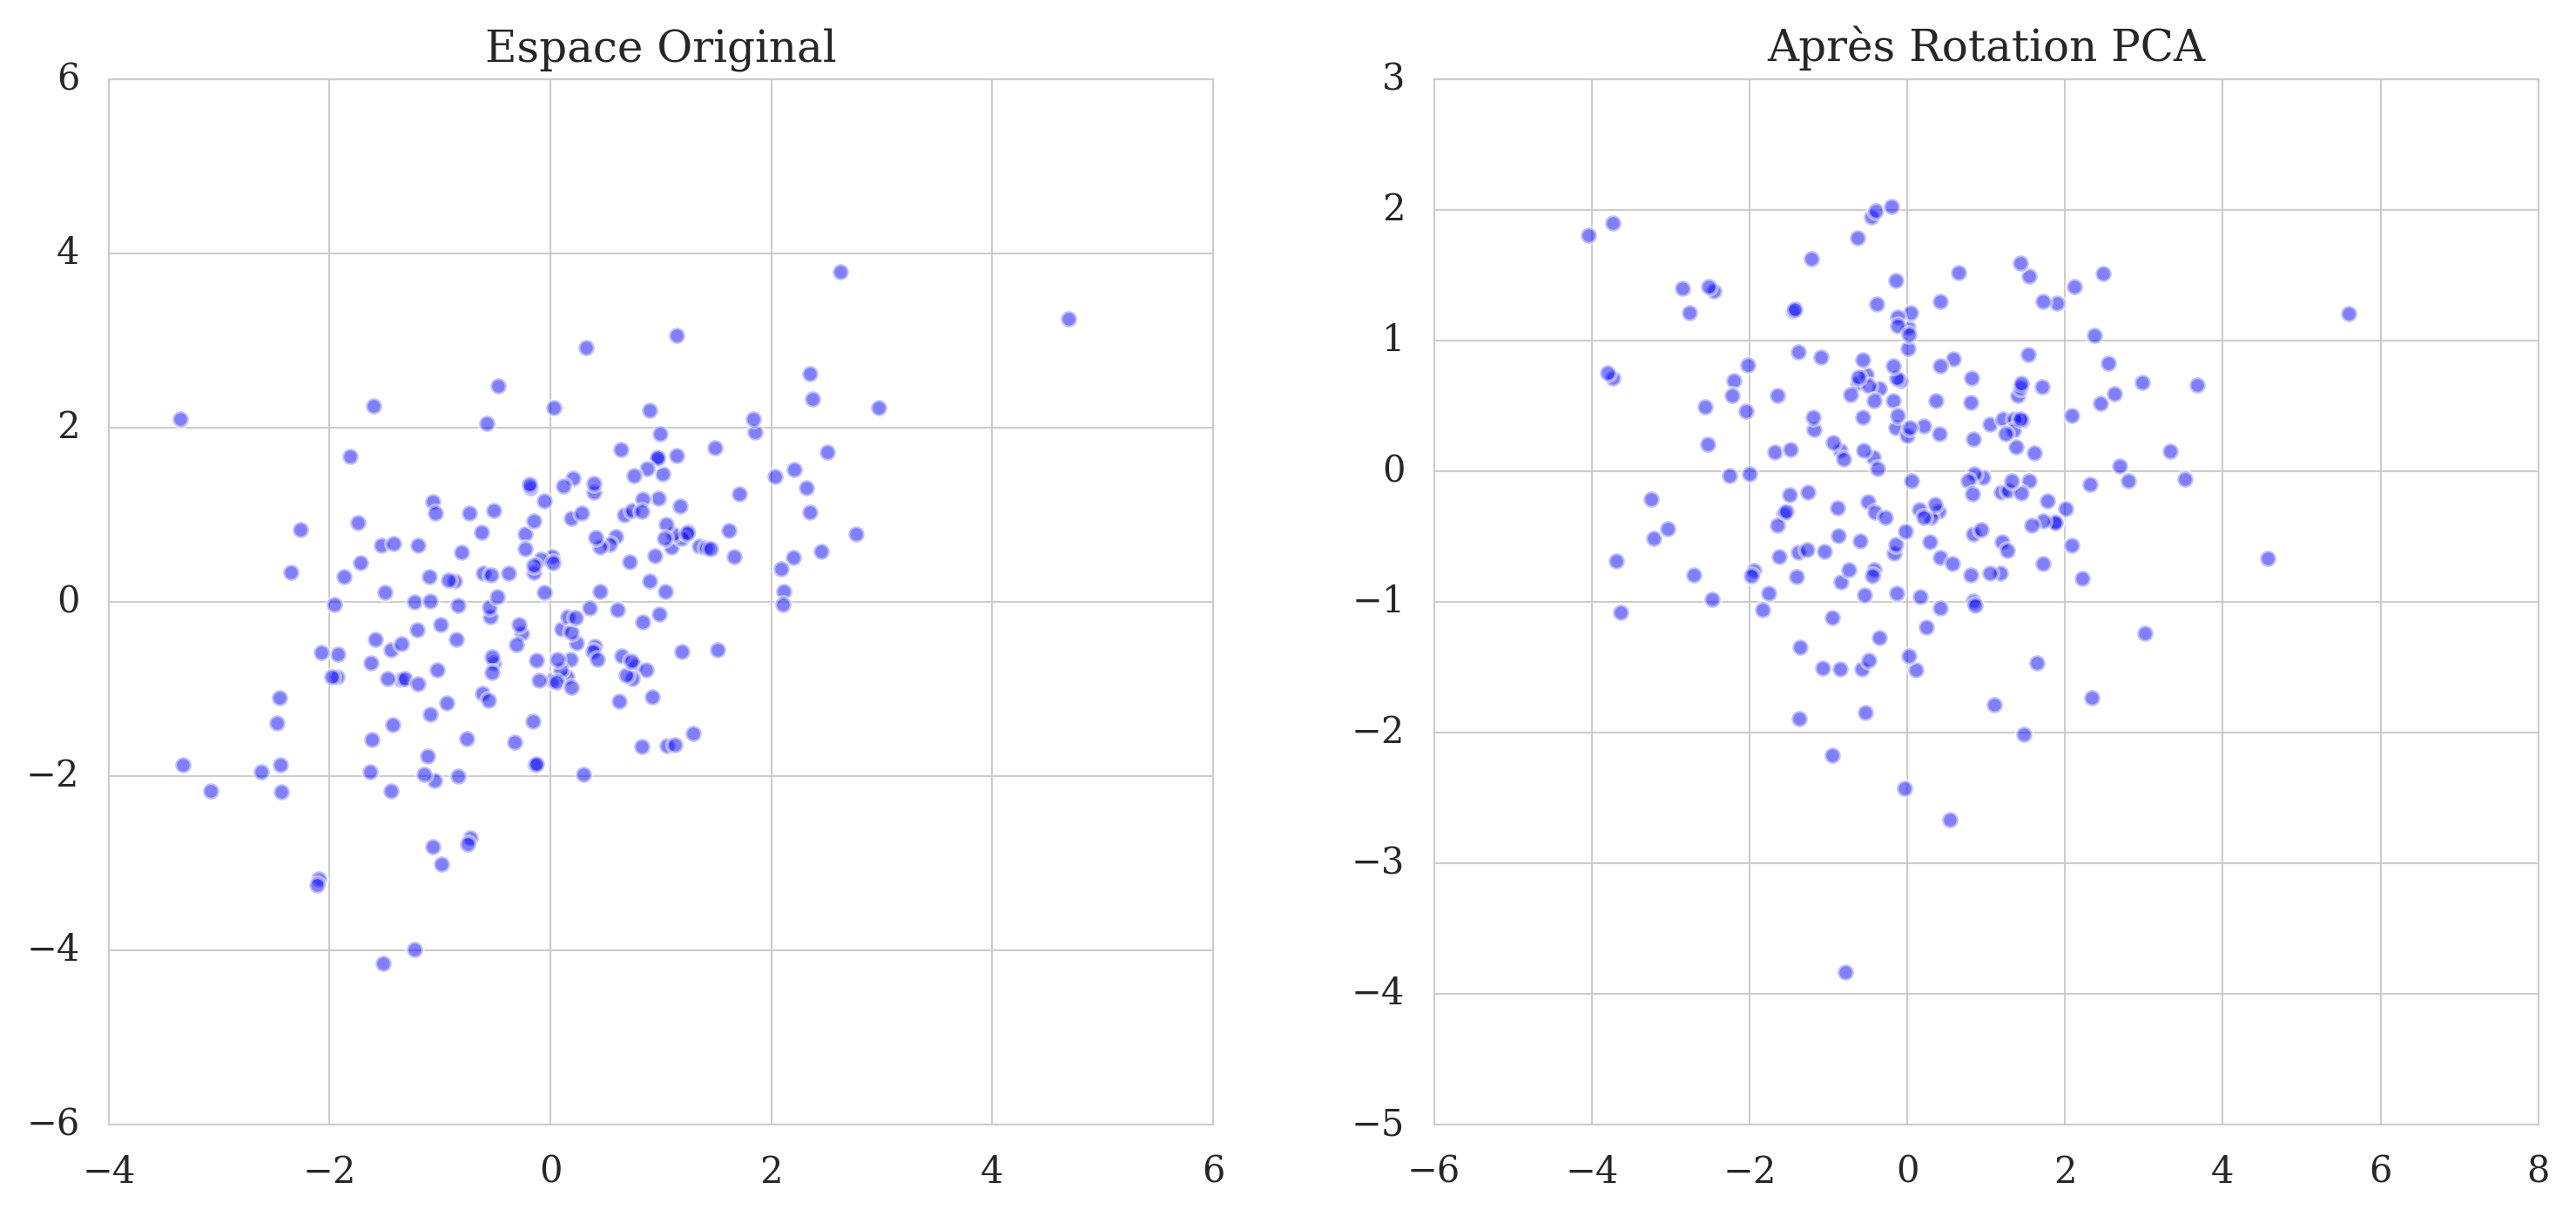
\includegraphics[width=0.8\textwidth]{pca_geometric.png}
    \caption{Interprétation géométrique de l'ACP comme rotation de l'espace}
    \label{fig:pca_geometric}
\end{figure}

\section{Limitations de l'ACP classique}

L'ACP, malgré sa puissance et sa popularité, présente plusieurs limitations importantes qu'il est crucial de comprendre pour une utilisation appropriée.

\subsection{Linéarité}
La limitation la plus fondamentale de l'ACP est son caractère linéaire. L'ACP ne peut capturer que des relations linéaires entre les variables.

\begin{figure}[H]
  \centering
  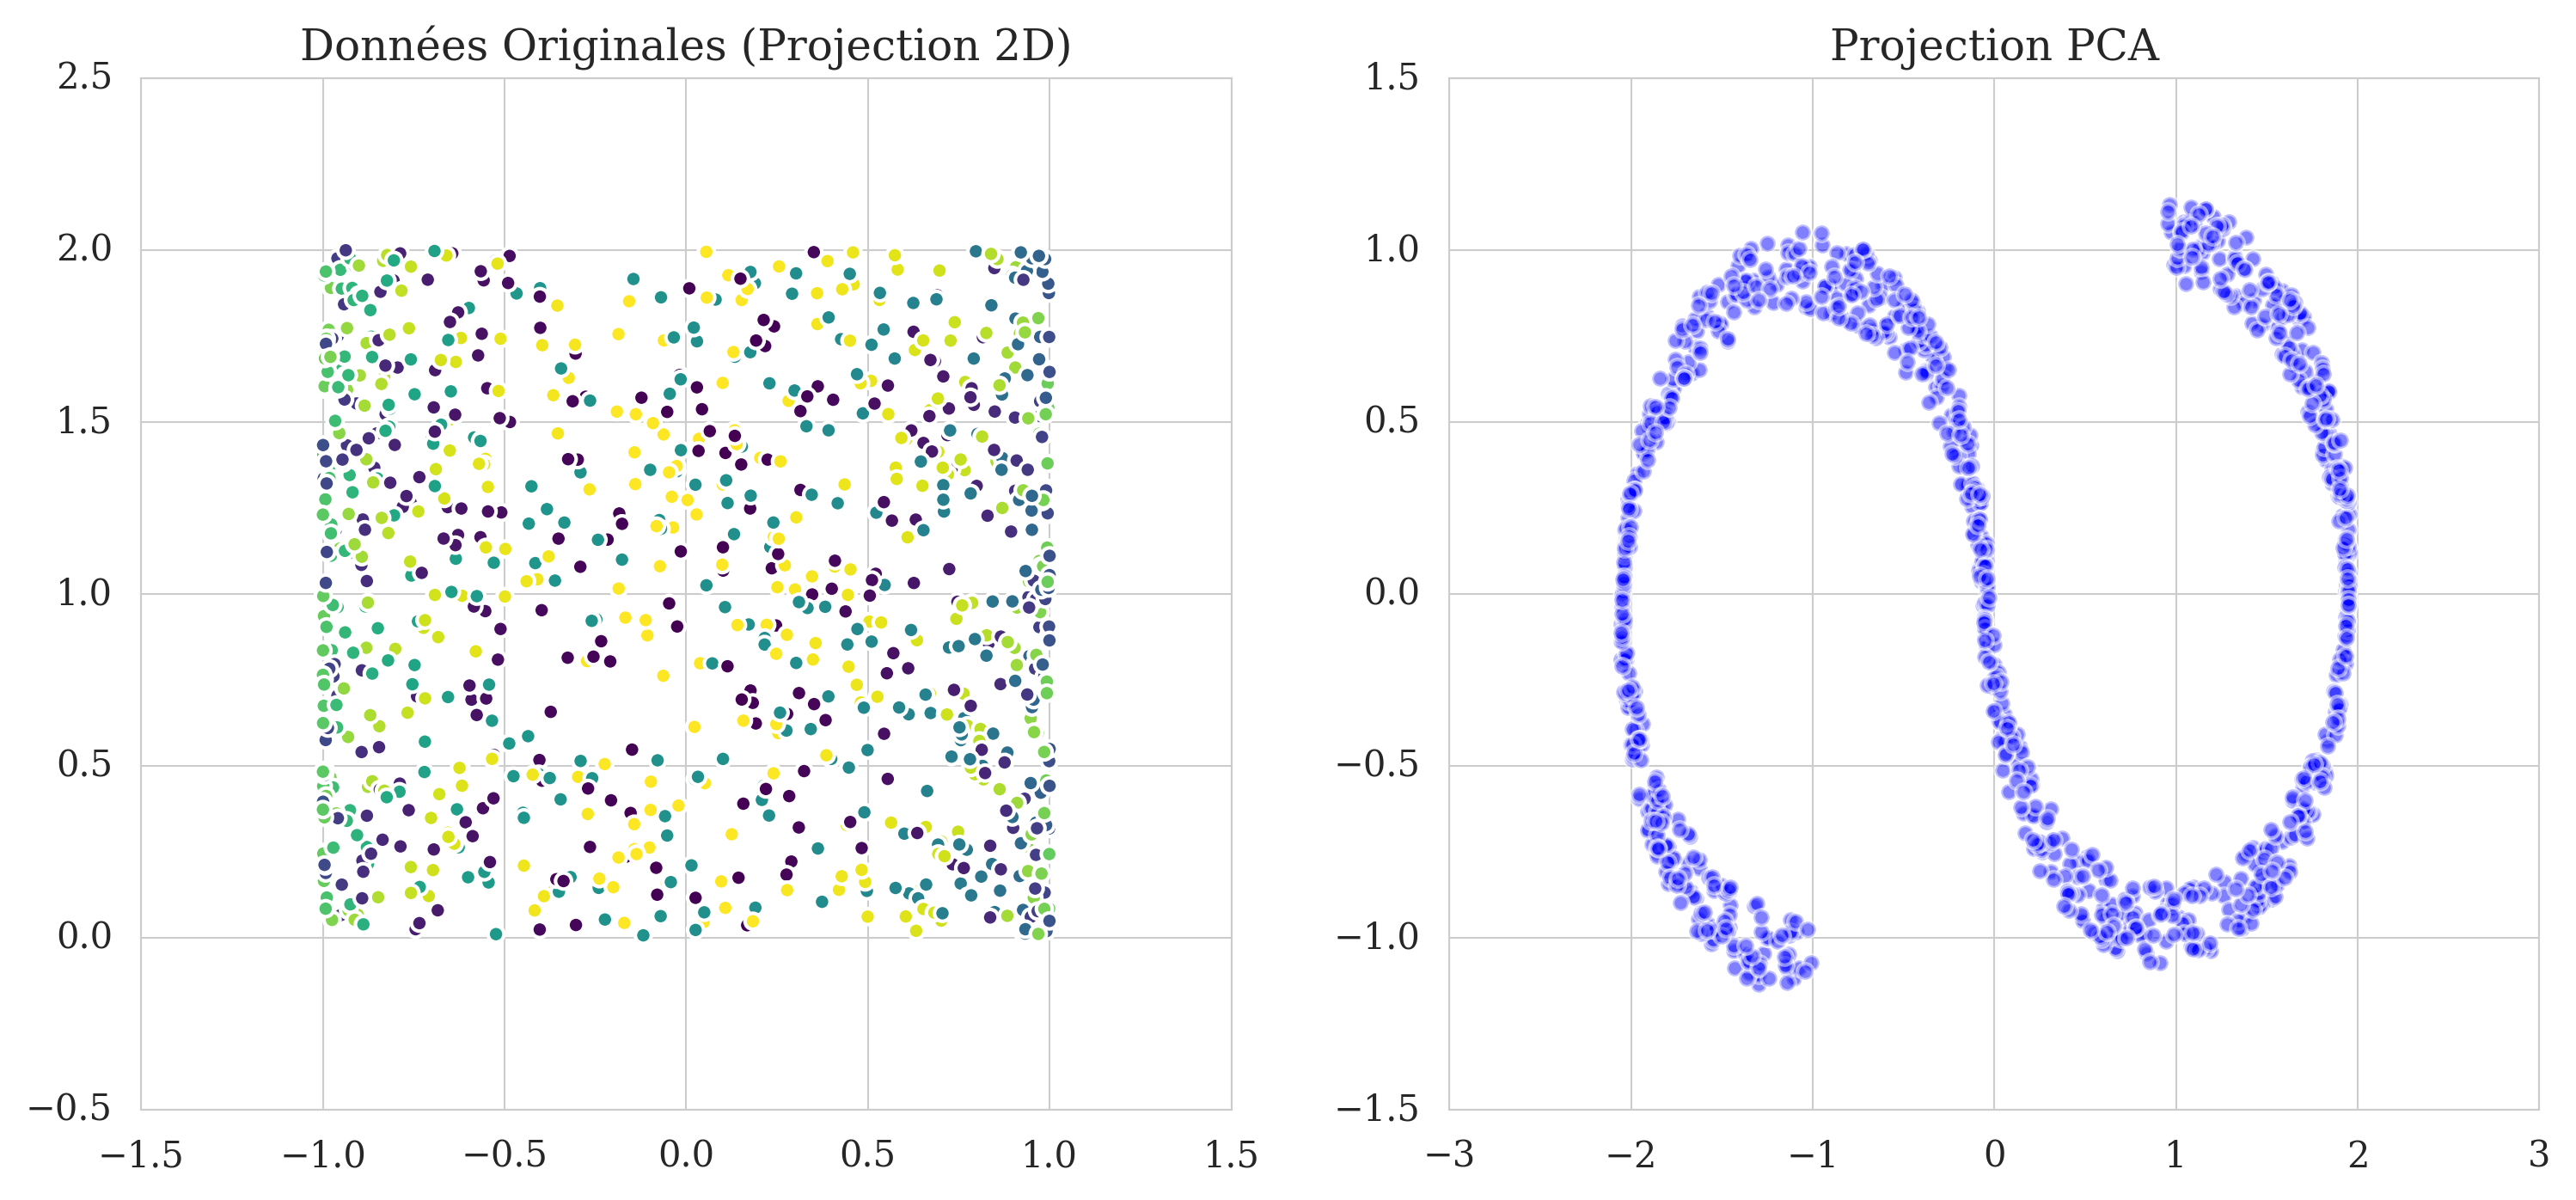
\includegraphics[width=1\textwidth]{nonlinear_pca_fail.png}
  \caption{Exemple de données non-linéaires où l'ACP échoue}
  \label{fig:nonlinear_fail}
\end{figure}

\textbf{Exemple concret :} Considérons des données disposées en spirale dans un espace 2D. L'ACP ne pourra pas "dérouler" cette spirale car elle ne peut effectuer que des transformations linéaires.

\subsection{Sensibilité aux valeurs aberrantes}
L'ACP classique est très sensible aux outliers car elle est basée sur la variance, qui elle-même est sensible aux valeurs extrêmes.

\begin{figure}[H]
  \centering
  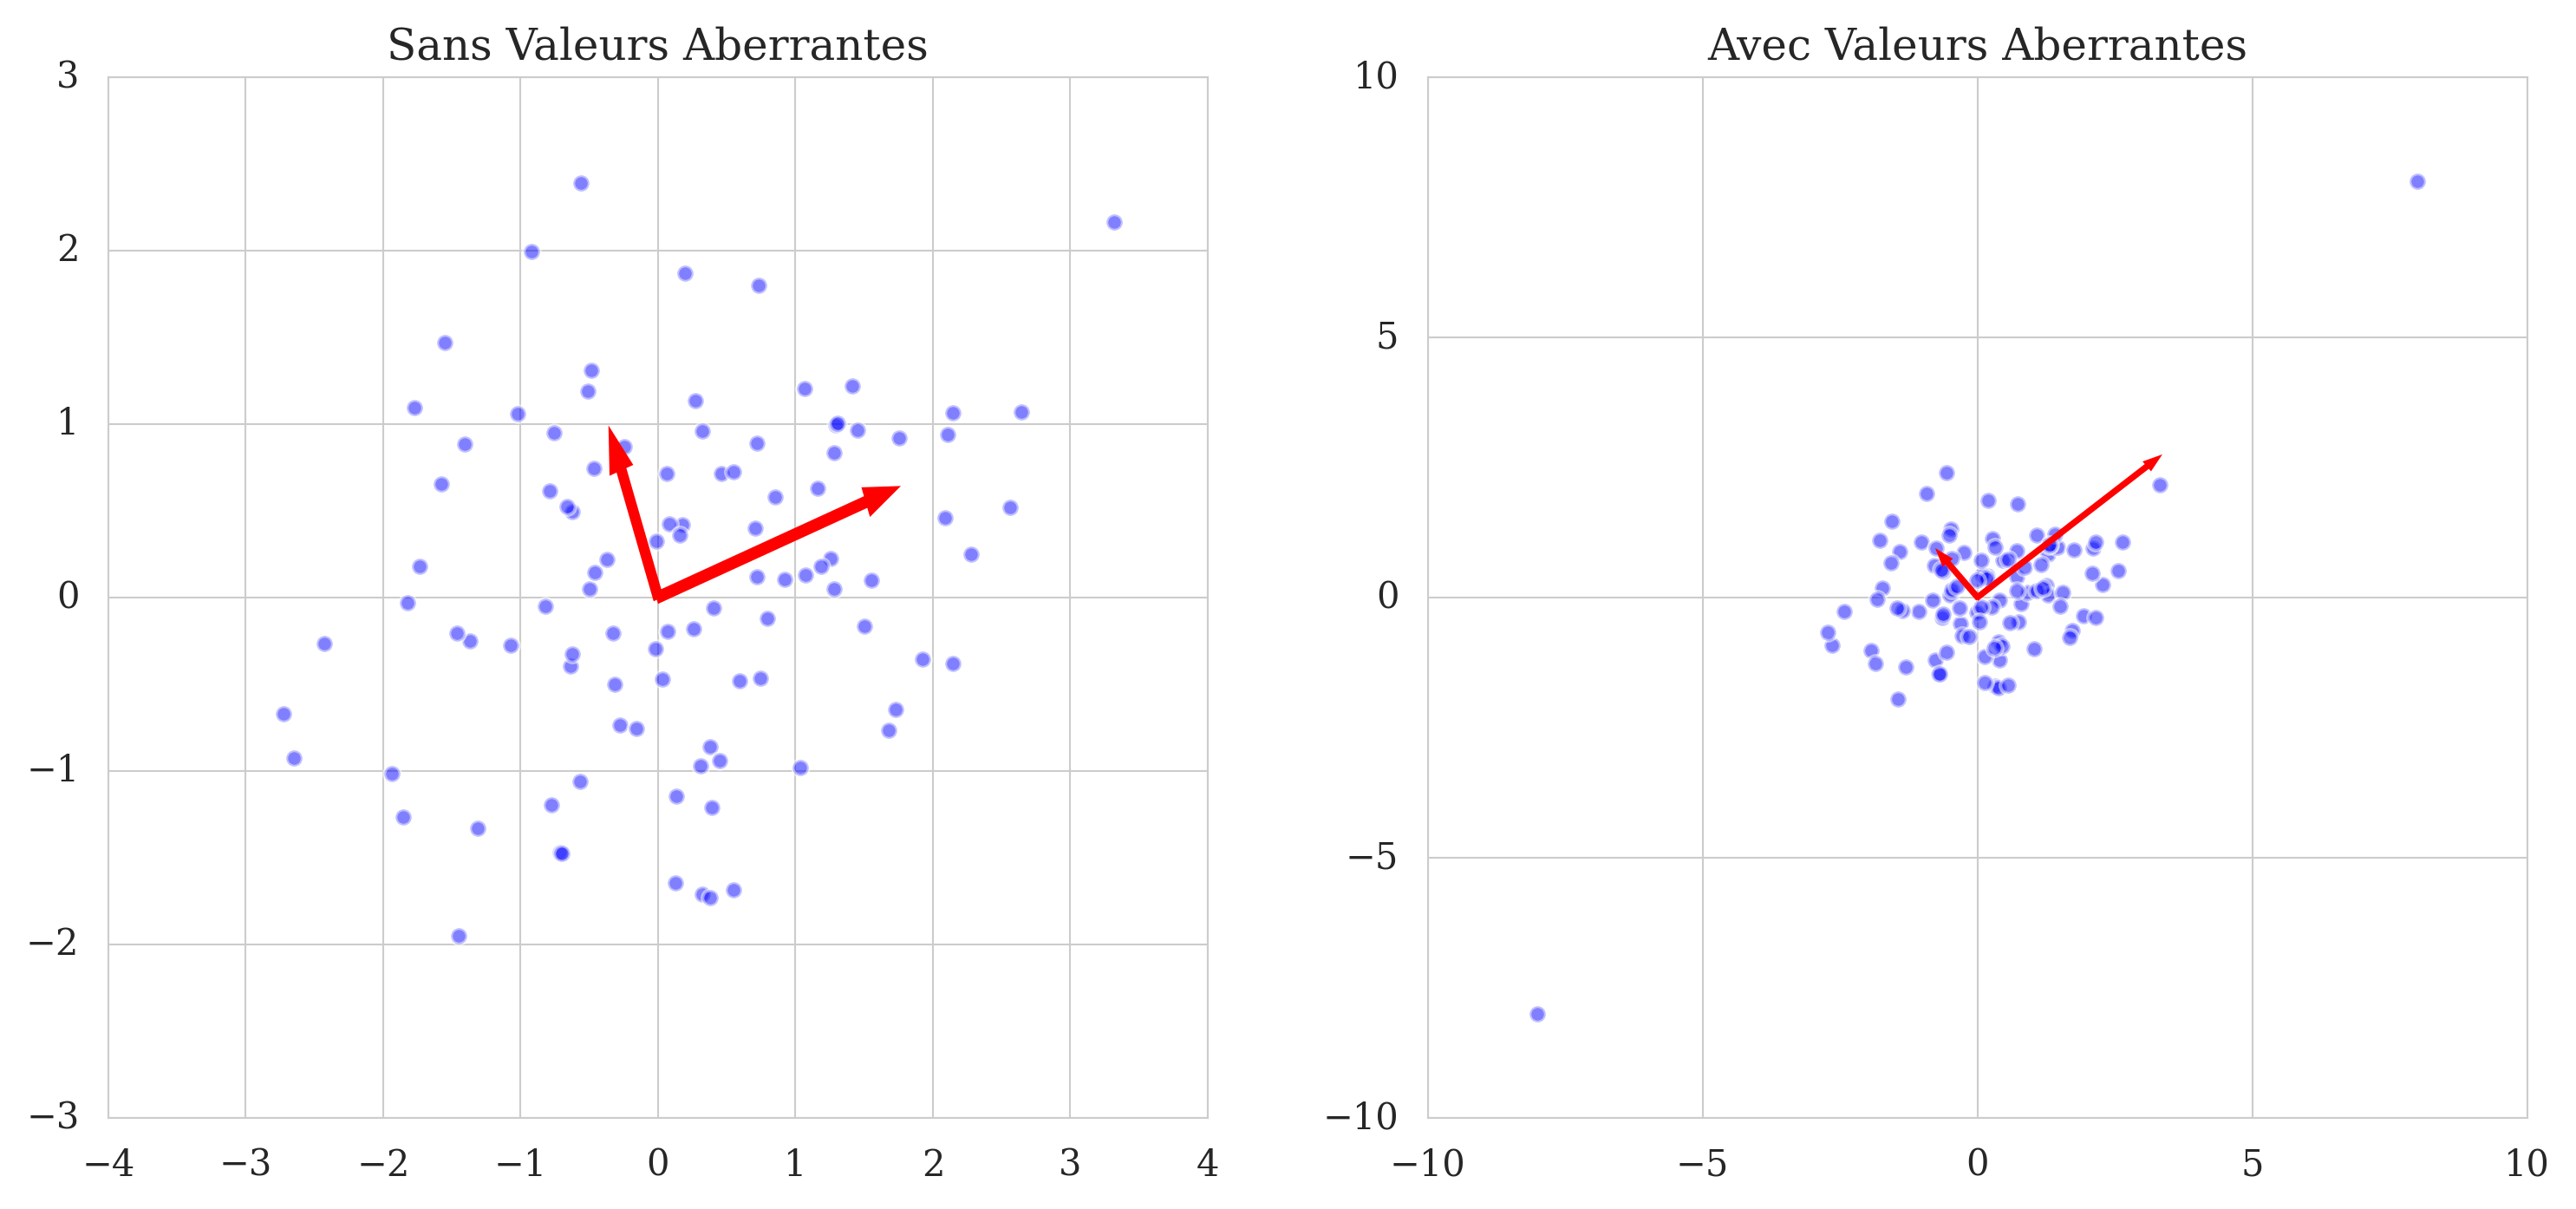
\includegraphics[width=1\textwidth]{outliers_impact.png}
  \caption{Impact des valeurs aberrantes sur les composantes principales}
  \label{fig:outliers_impact}
\end{figure}

\textbf{Exemple numérique :} Dans un jeu de données financières, un seul point aberrant (comme un crash boursier) peut complètement modifier l'orientation des composantes principales.

\subsection{Hypothèse de normalité}
L'ACP suppose implicitement que les données suivent une distribution normale multivariée, ce qui n'est pas toujours le cas en pratique.

\textbf{Exemple :} Dans l'analyse de données de consommation électrique, les distributions sont souvent asymétriques avec des pics aux heures de pointe.

\subsection{Perte d'interprétabilité}
Les composantes principales sont des combinaisons linéaires de toutes les variables originales, ce qui peut rendre leur interprétation difficile.

\textbf{Exemple pratique :}
Dans une étude médicale avec 100 mesures différentes, chaque composante principale pourrait impliquer toutes ces mesures avec des coefficients non nuls, rendant l'interprétation clinique complexe.

\subsection{Solutions alternatives}
Pour remédier à ces limitations, plusieurs variantes ont été développées :

\begin{itemize}
  \item \textbf{Kernel PCA} : Pour traiter les relations non-linéaires
  \item \textbf{Robust PCA} : Pour gérer les valeurs aberrantes
  \item \textbf{Sparse PCA} : Pour améliorer l'interprétabilité
  \item \textbf{Probabilistic PCA} : Pour prendre en compte l'incertitude
\end{itemize}

\begin{table}[H]
  \centering
  \begin{tabular}{|l|l|l|}
    \hline
    \textbf{Limitation} & \textbf{Impact} & \textbf{Solution} \\
    \hline
    Linéarité & Mauvaise capture des relations non-linéaires & Kernel PCA \\
    Outliers & Distorsion des composantes & Robust PCA \\
    Interprétabilité & Difficulté d'analyse & Sparse PCA \\
    Normalité & Biais sur données non-gaussiennes & Probabilistic PCA \\
    \hline
  \end{tabular}
  \caption{Résumé des limitations et solutions}
\end{table}


Cette compréhension des limitations de l'ACP est essentielle pour choisir la variante appropriée selon le contexte d'application et la nature des données analysées.

\newpage

\chapter{Application pratique de l'ACP}
\label{chap:acp_compression}

\section{Réduction de dimension et qualité visuelle}
\label{sec:acp_images}

L’Analyse en Composantes Principales (ACP) permet de projeter une image haute
définition dans un espace latent de dimension beaucoup plus faible tout en
préservant l’essentiel de l’information perceptuelle.

\begin{figure}[H]
  \centering
    
  \begin{subfigure}{0.18\textwidth}
    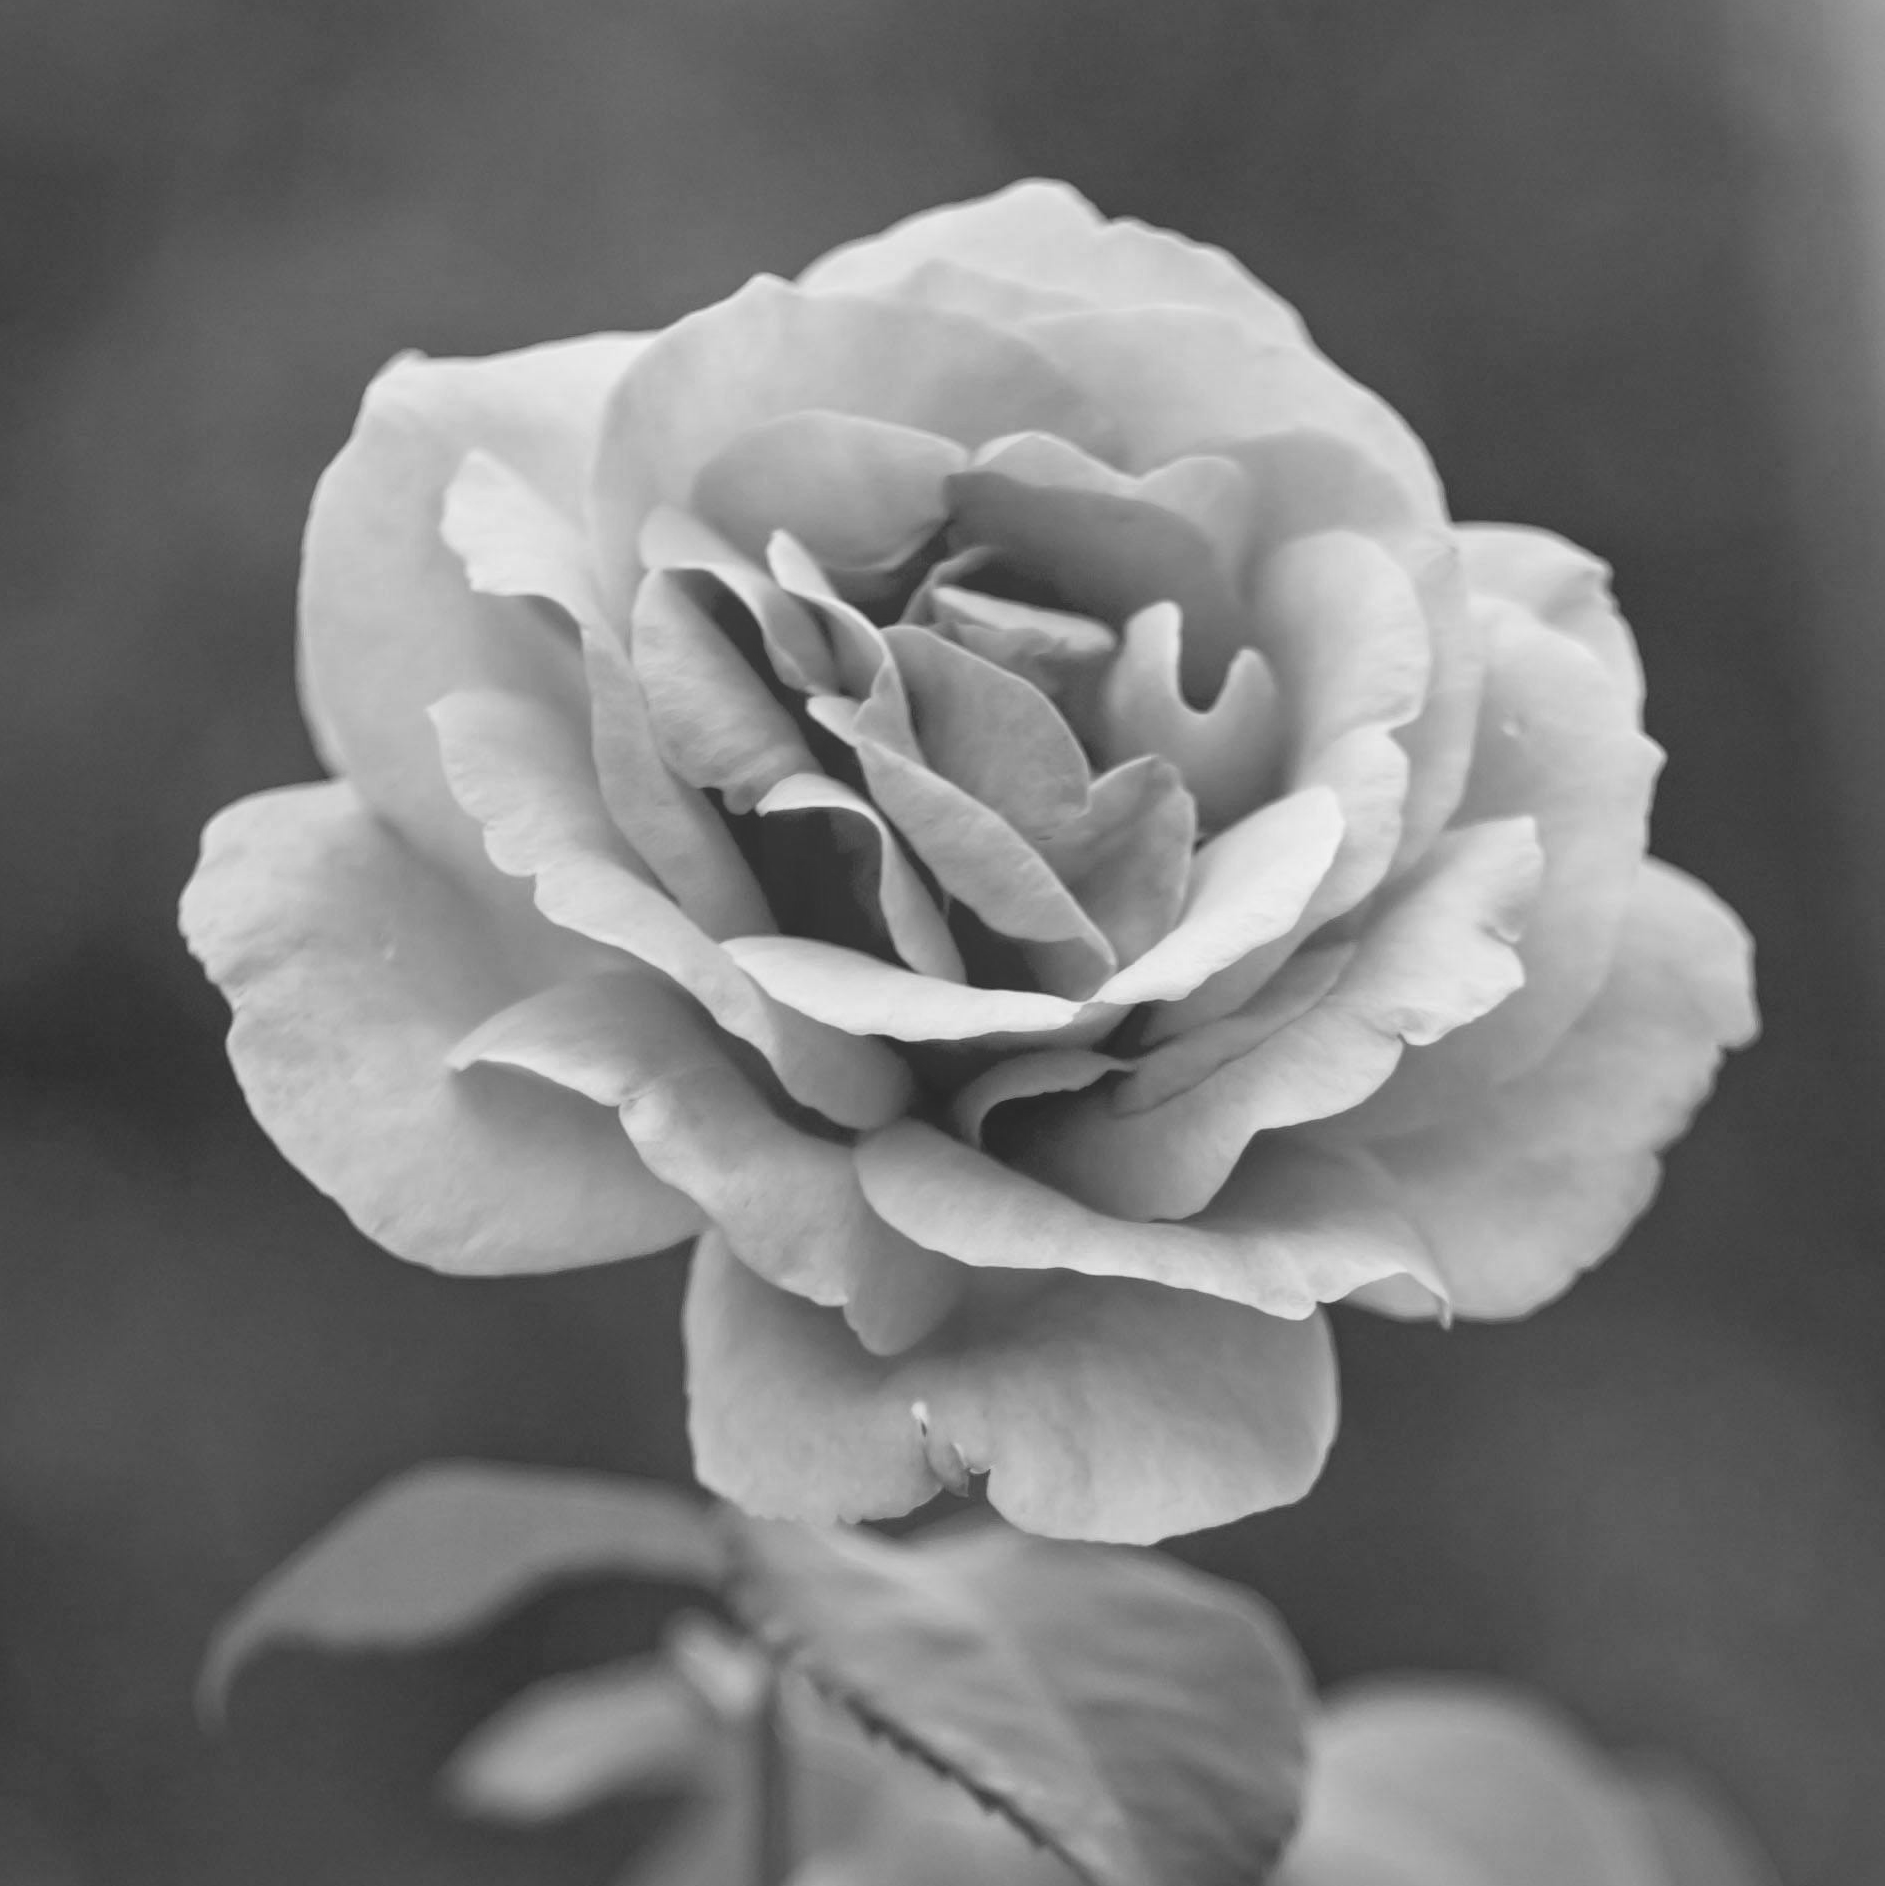
\includegraphics[width=\linewidth]{images/original.png}
    \caption*{Original}
  \end{subfigure}\hfill
  \begin{subfigure}{0.18\textwidth}
    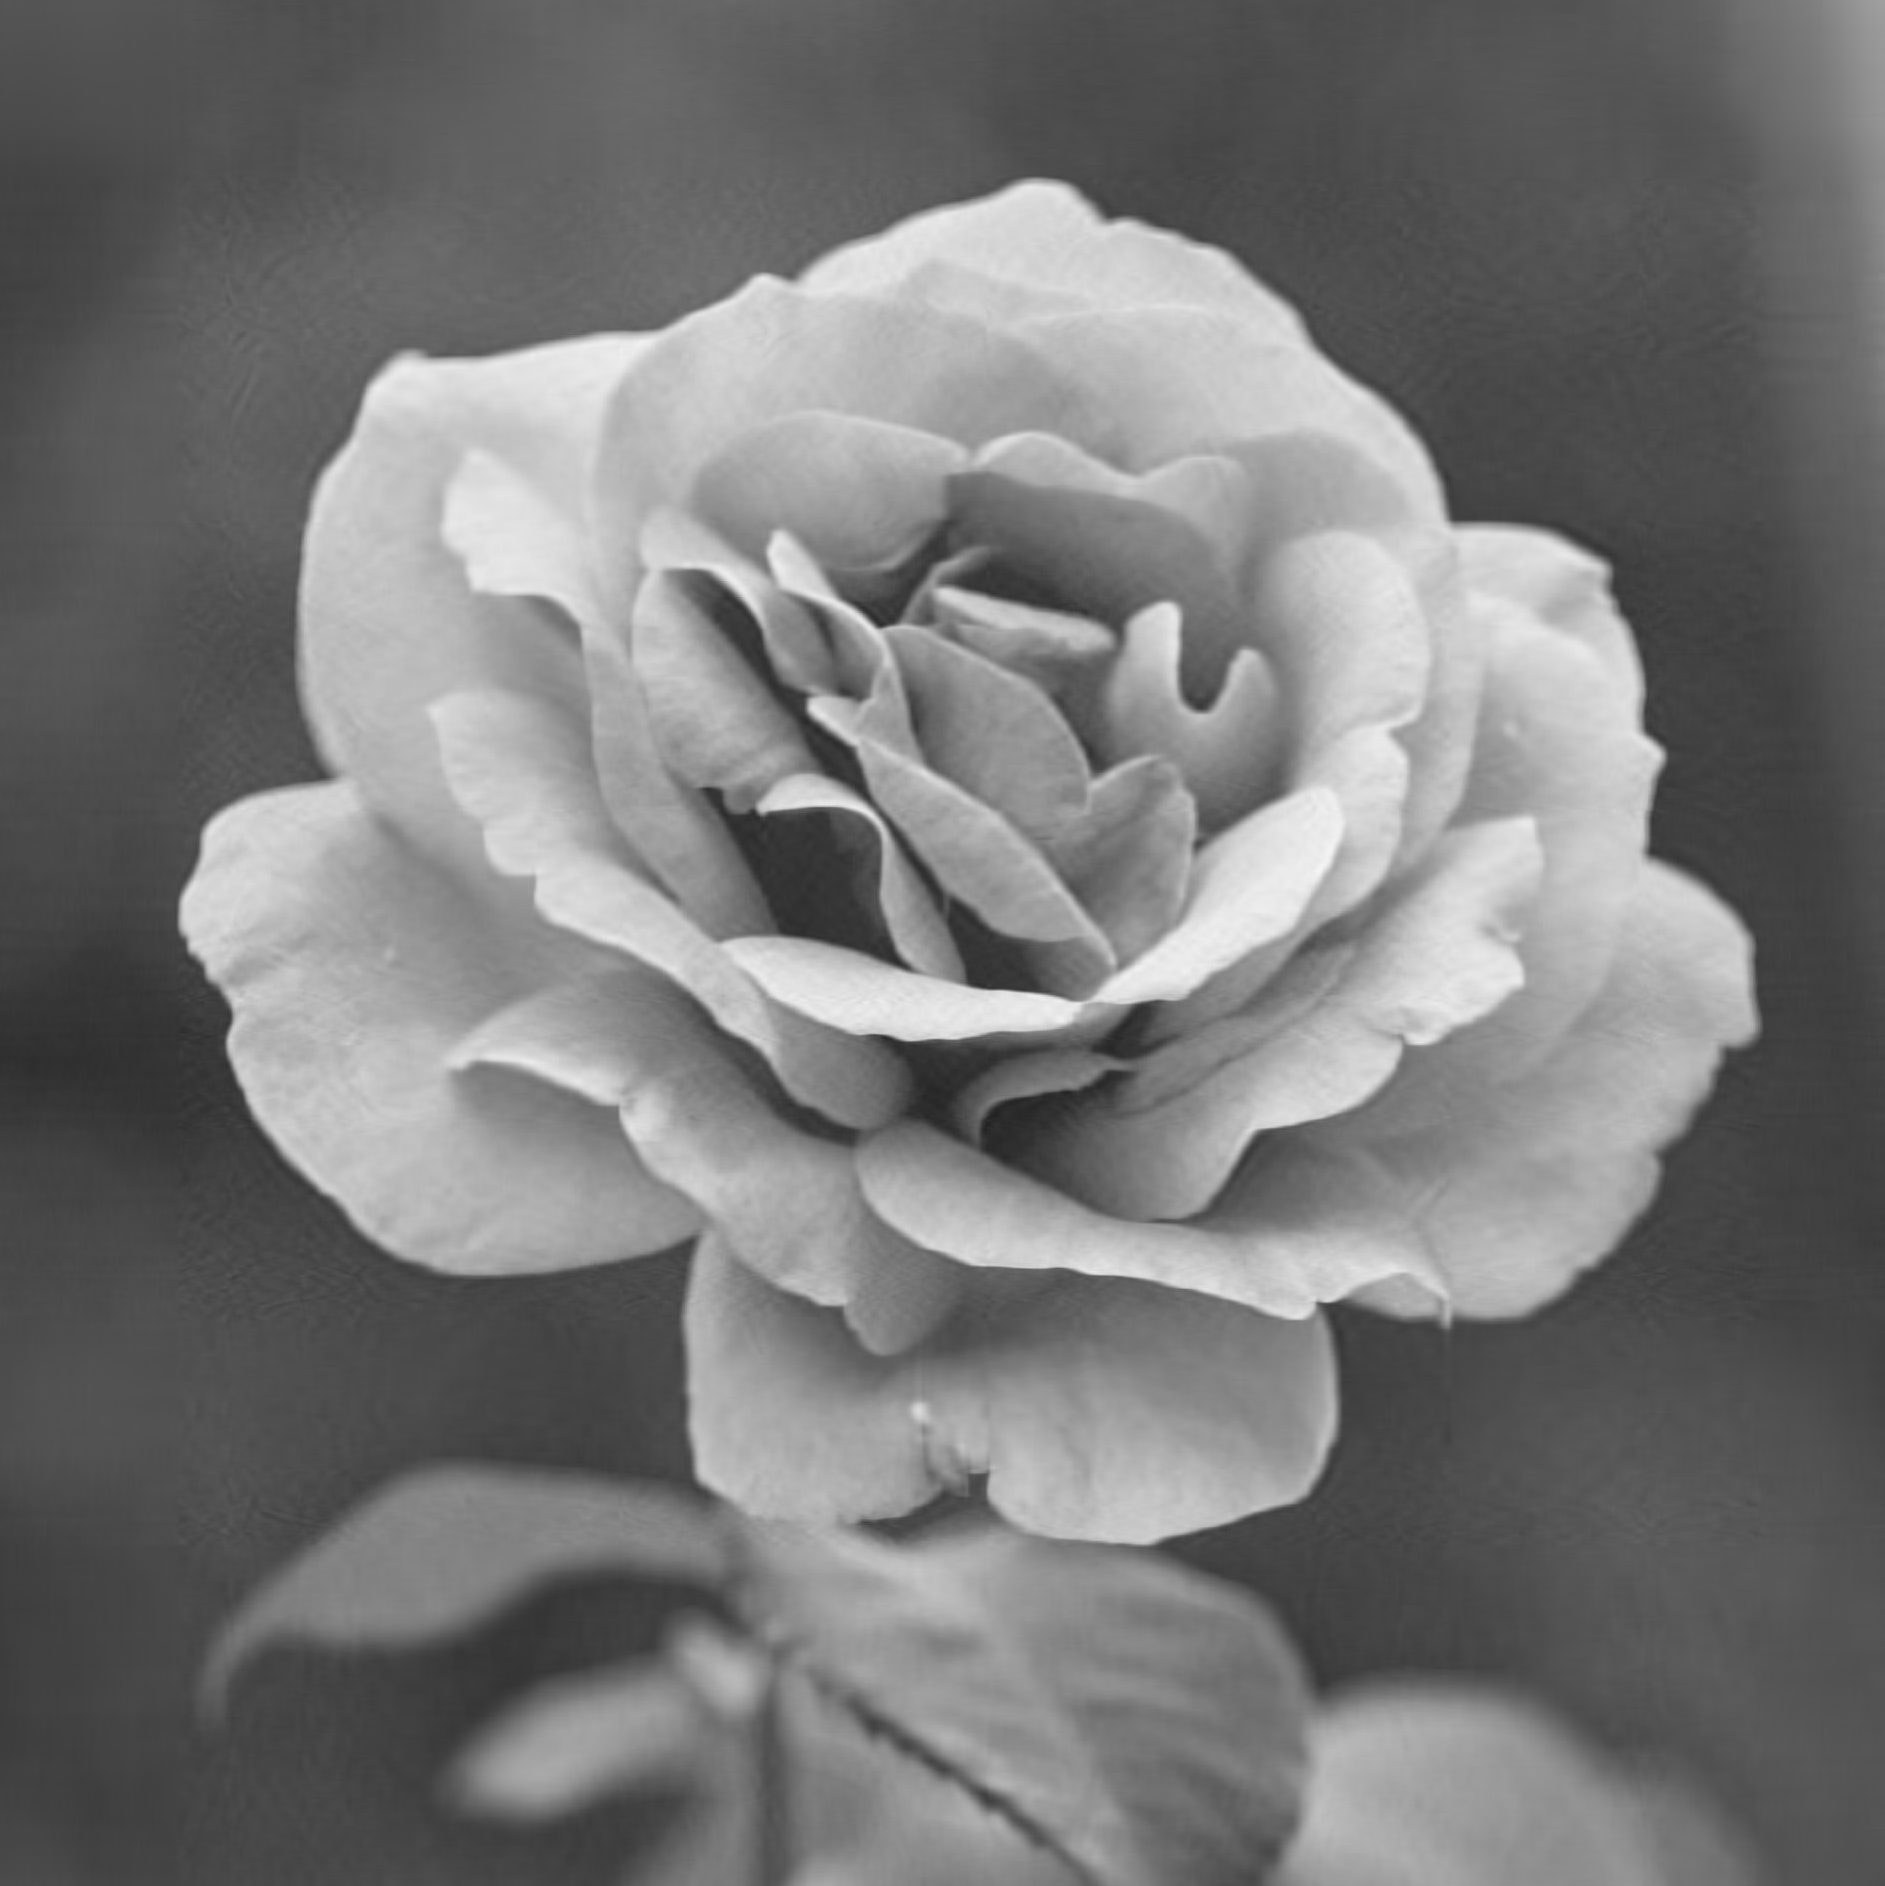
\includegraphics[width=\linewidth]{images/pca_100.png}
    \caption*{100 composantes}
  \end{subfigure}\hfill
  \begin{subfigure}{0.18\textwidth}
    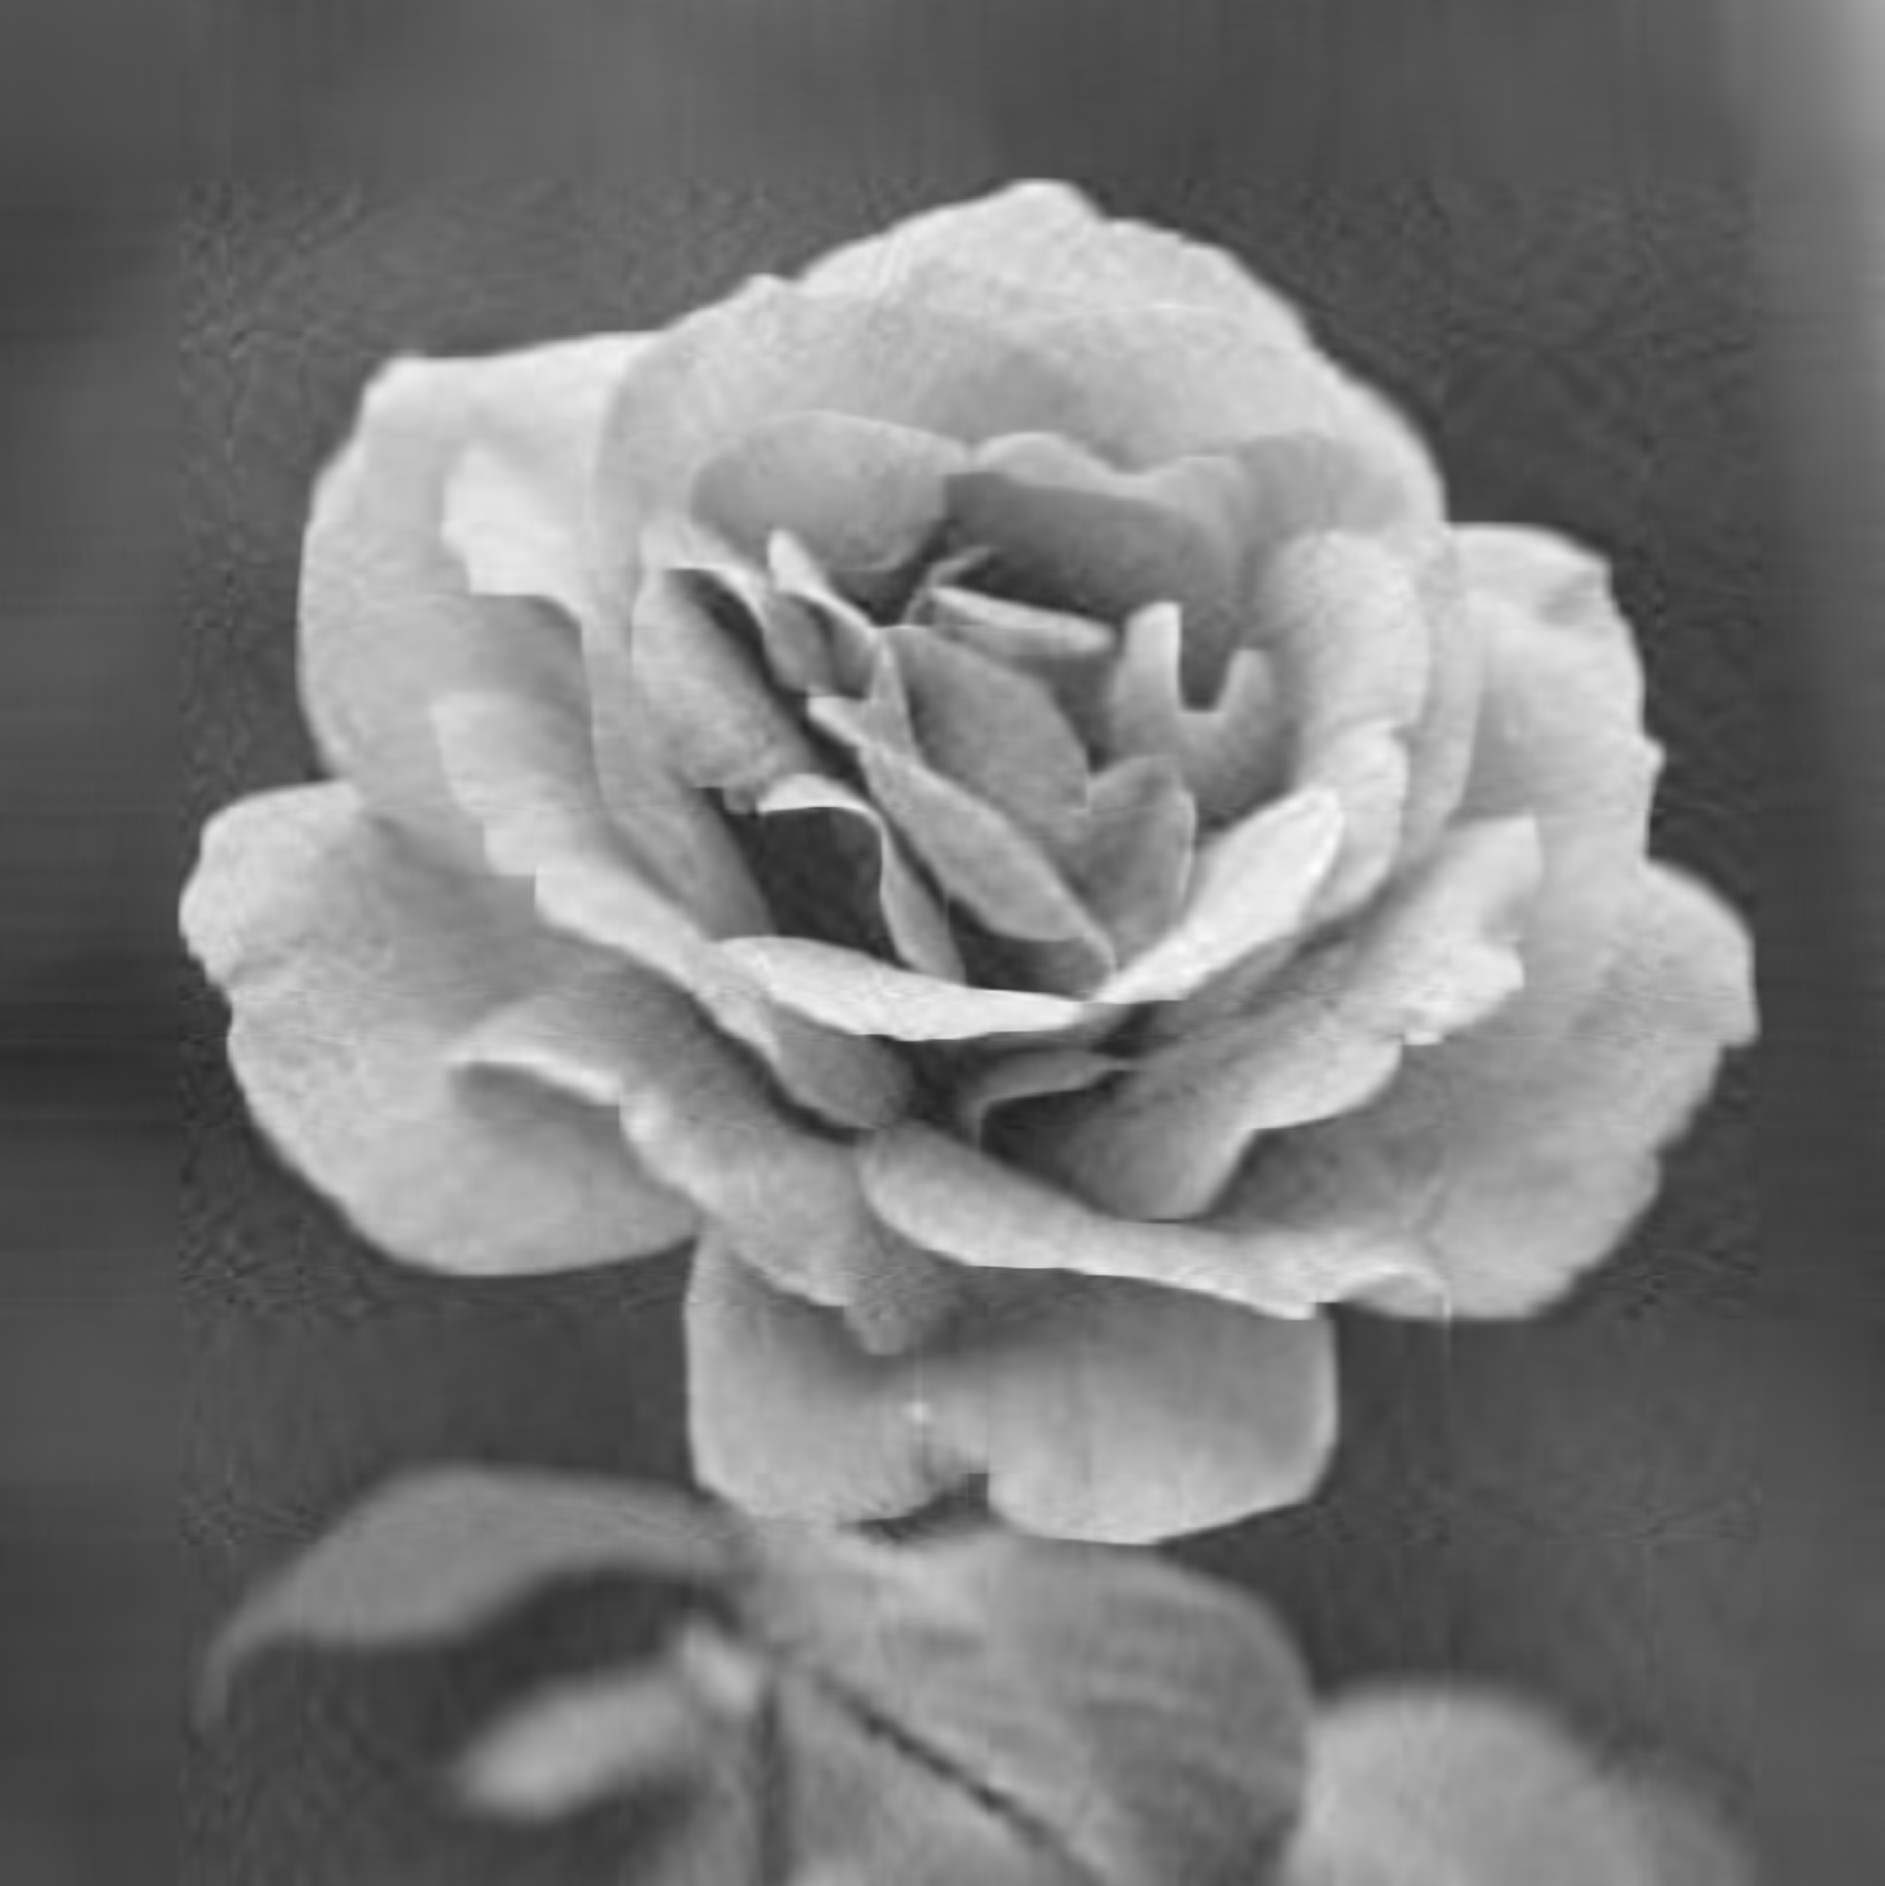
\includegraphics[width=\linewidth]{images/pca_50.png}
    \caption*{50 composantes}
  \end{subfigure}\hfill
  \begin{subfigure}{0.18\textwidth}
    
\includegraphics[width=\linewidth]{images/pca_25.png}
    \caption*{25 composantes}
  \end{subfigure}\hfill
  \begin{subfigure}{0.18\textwidth}
    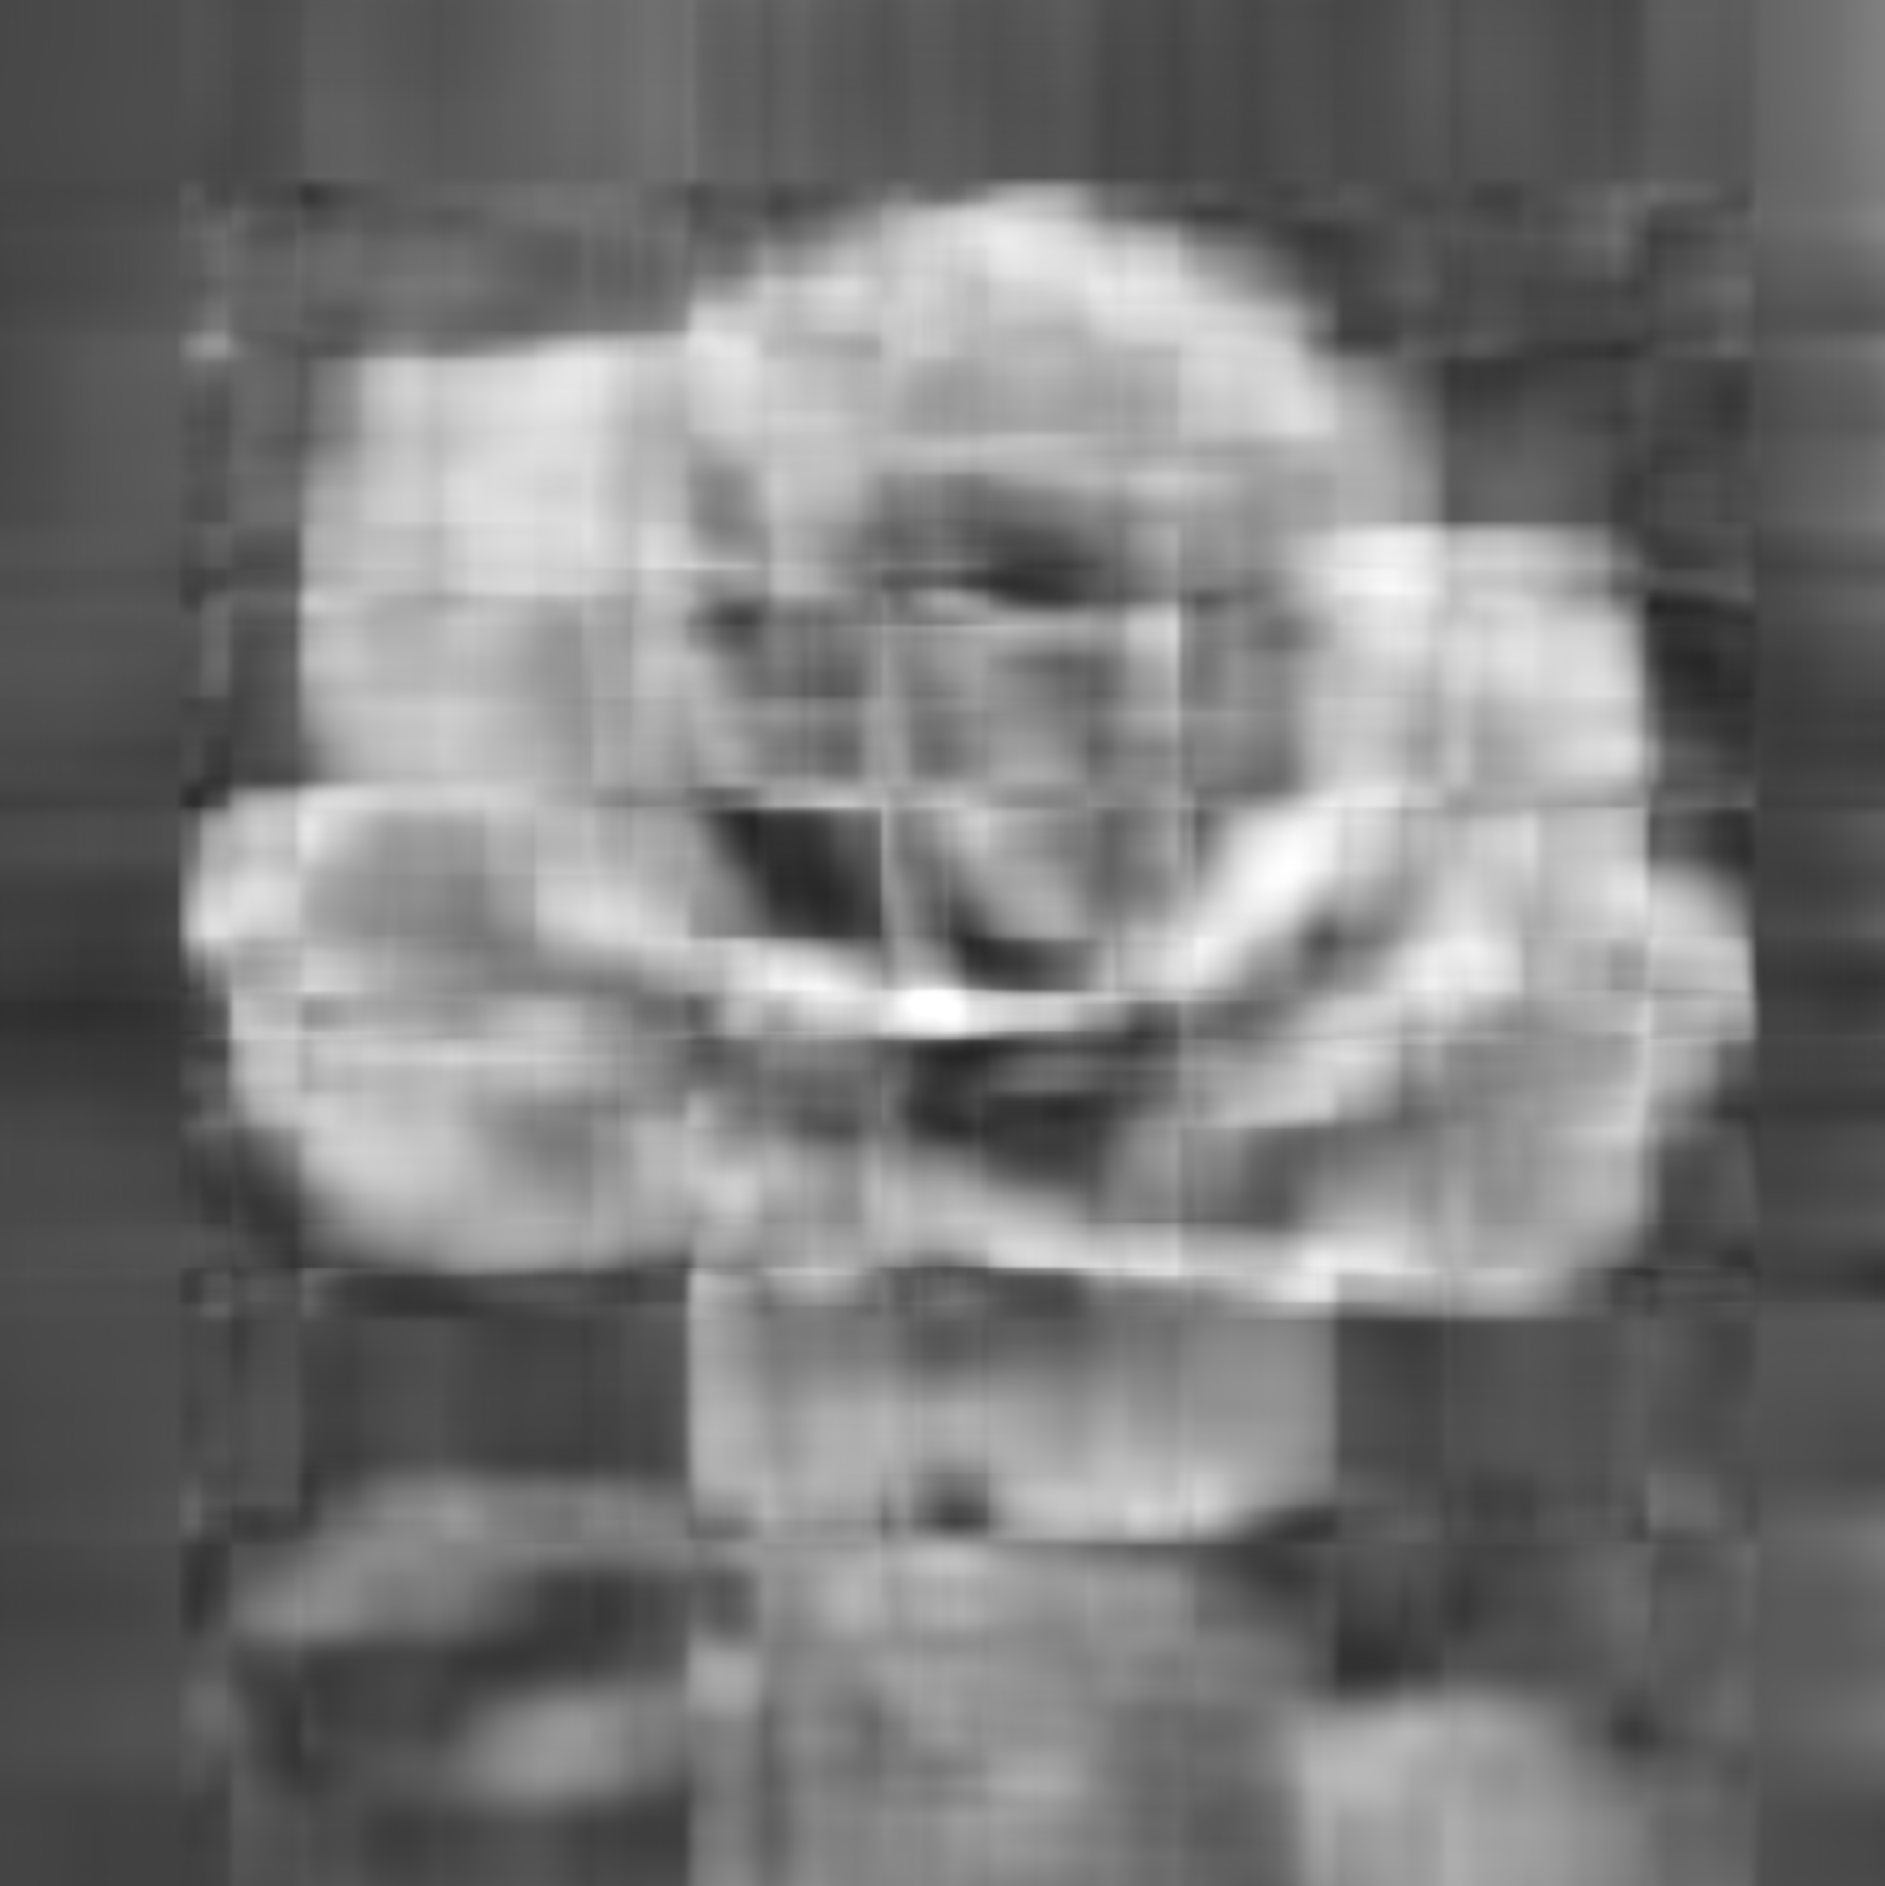
\includegraphics[width=\linewidth]{images/pca_10.png}
    \caption*{10 composantes}
  \end{subfigure}
  \caption{Effet du nombre de composantes principales \(k\) sur la qualité visuelle.}
  \label{fig:acp_degraded}
\end{figure}

La Figure~\ref{fig:acp_degraded} illustre la dégradation graduelle : on passe
de l’image originale (vecteur de dimension \(n\)) à des reconstructions
respectivement sur \(k=100\), \(50\), \(25\) et \(10\) dimensions.  
La Figure~\ref{fig:acp_curve} synthétise l’évolution conjointe
\emph{taille \(\rightarrow\) qualité}. On observe qu’entre \(k=25\) et \(k=50\),
le gain en qualité devient marginal alors que la taille double.

\begin{figure}[H]
  \centering
    
  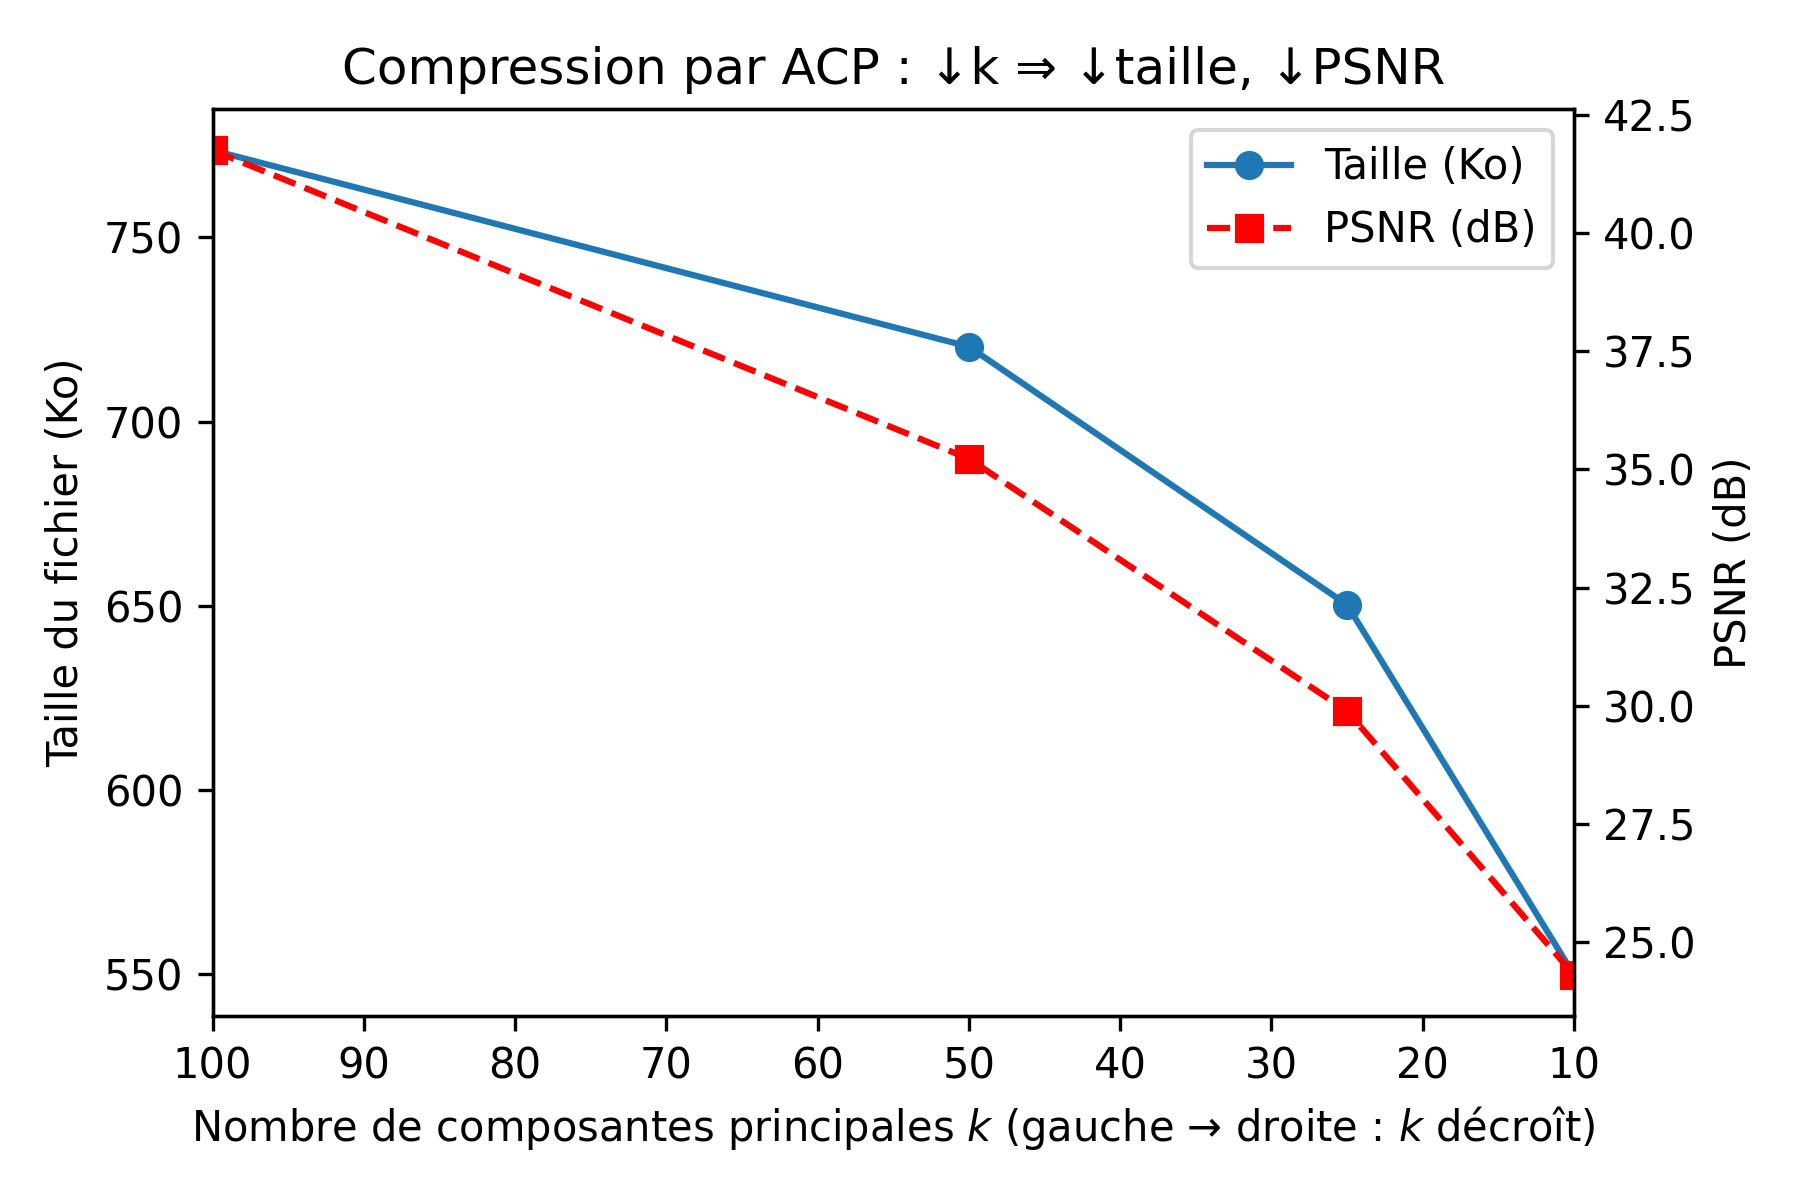
\includegraphics[width=0.75\textwidth]{images/pca_storage_vs_quality.png}
  \caption{Relation entre le nombre de composantes \(k\), la taille de fichier
           (Ko) et la qualité de reconstruction (PSNR en dB).}
  \label{fig:acp_curve}
\end{figure}


\section{Eigenfaces : Méthode de Reconnaissance Faciale}
\begin{itemize}
  \item On dispose d’un ensemble d’images de visages alignées et centrées.
  \item Chaque image $I$ est convertie en vecteur de pixels, puis centrée :
    \[
      I_{\mathrm{centr\acute{e}}} = I - I_{\mathrm{mean}}.
    \]
  \item L’ACP est appliquée à la matrice de données de dimension $n \times p$ (images × pixels).
\end{itemize}

\section{Rôle central de l’ACP dans Eigenfaces}
Soit un ensemble de $n$ images vectorisées $I_1,\dots,I_n\in\mathbb{R}^p$, et leur moyenne
\[
  I_{\mathrm{mean}} = \frac{1}{n} \sum_{i=1}^n I_i.
\]
Définissons la matrice de données centrée
\[
  X = \bigl[I_1 - I_{\mathrm{mean}},\;\dots,\;I_n - I_{\mathrm{mean}}\bigr] \in \mathbb{R}^{p\times n}.
\]

Tout visage $I$ s'encode alors par les coefficients
\[
  z = W^{\top}(I - I_{\mathrm{mean}}) \in \mathbb{R}^K,
\]
assurant :
\begin{itemize}
  \item réduction de dimension : $p\to K\ll p$,  
  \item filtrage du bruit : on supprime les composantes de faible variance,  
  \item extraction des traits dominants : chaque $w_i$ capture une “direction” de variation.
\end{itemize}

\chapter{Analyse des résultats}

\section{Indice SSIM et application à l’ACP}

\subsection*{Principe du SSIM}

L’objectif du SSIM (\textit{Structural Similarity Index}) est de quantifier la similarité \emph{perçue} entre deux images.

\subsubsection*{Composantes du SSIM}

Le SSIM est défini localement, généralement sur une fenêtre de taille $11 \times 11$, à partir de trois composantes :

\begin{equation}
  \mathrm{SSIM}(x,y) = 
  \underbrace{l(x,y)}_{\text{luminance}} \times 
  \underbrace{c(x,y)}_{\text{contraste}} \times 
  \underbrace{s(x,y)}_{\text{structure}}
\end{equation}

Ces composantes sont calculées par :
\begin{align}
  l(x,y) &= \frac{2\mu_x\mu_y + C_1}{\mu_x^2 + \mu_y^2 + C_1}, \\
  c(x,y) &= \frac{2\sigma_x\sigma_y + C_2}{\sigma_x^2 + \sigma_y^2 + C_2}, \\
  s(x,y) &= \frac{\sigma_{xy} + C_3}{\sigma_x\,\sigma_y + C_3}.
\end{align}

Le SSIM prend ses valeurs dans l’intervalle $[-1,1]$ :
\begin{itemize}
  \item $1$ : images identiques,
  \item $0$ : aucune corrélation perceptible.
\end{itemize}

\subsection*{Application du SSIM à l’ACP}

\begin{enumerate}
  \item \textbf{Compression par ACP}
    \begin{itemize}
      \item Réduction de dimension des images (vectorisation).
      \item Reconstruction avec les $k$ premières composantes principales.
    \end{itemize}

  \item \textbf{Évaluation par SSIM}
    \begin{itemize}
      \item Calcul du SSIM entre l’image originale et l’image reconstruite.
      \item Tracé du SSIM en fonction de $k$ pour étudier le compromis qualité vs. taille.
    \end{itemize}

  \item \textbf{Sélection adaptative}  
    Choix du plus petit $k$ tel que $\mathrm{SSIM}\ge0{,}95$.

  \item \textbf{Critère d’arrêt}  
    Arrêt de l’ajout de composantes dès que $\Delta \mathrm{SSIM} < \varepsilon$.
\end{enumerate}

\section{Calcul des moyennes locales $\mu_x$ et $\mu_y$}

\begin{itemize}
  \item Fenêtre courante : $11 \times 11$ ou $8 \times 8$ pixels.
  \item Pondération par filtre gaussien 2D ($\sigma \approx 1{,}5$) :
    \[
      \mu_x(i,j) = \sum_{u,v}w(u,v)\,X(i+u,j+v),\quad
      \mu_y(i,j) = \sum_{u,v}w(u,v)\,Y(i+u,j+v).
    \]
  \item Implémentation rapide : convolution ou \texttt{cv2.GaussianBlur}.
\end{itemize}

\subsection*{Exemple Python (OpenCV)}

\begin{verbatim}
mu_x = cv2.GaussianBlur(X, (11, 11), 1.5)
mu_y = cv2.GaussianBlur(Y, (11, 11), 1.5)
\end{verbatim}

\section{Constantes $C_1$, $C_2$, $C_3$}

\subsection*{Définitions générales}

\[
  C_1 = (K_1\,L)^2,\quad
  C_2 = (K_2\,L)^2,\quad
  C_3 = \frac{C_2}{2}.
\]

\subsection*{Valeurs usuelles}

\begin{itemize}
  \item $L$ : dynamique (8 bits $\to$ 255, normalisé $\to$ 1).
  \item Biens conseillés : $K_1=0{,}01$, $K_2=0{,}03$.
  \item \textbf{Images 8 bits} ($L=255$) :  
    $C_1\approx6{,}5025,\;C_2\approx58{,}5225,\;C_3\approx29{,}2612$.
  \item \textbf{Images normalisées} ($L=1$) :  
    $C_1=1\times10^{-4},\;C_2=9\times10^{-4},\;C_3=4{,}5\times10^{-4}$.
\end{itemize}

\subsection*{À retenir}

\begin{itemize}
  \item $\mu_x,\mu_y$ : moyennes locales via filtre gaussien.
  \item $C_1,C_2,C_3$ : stabilisation des divisions.
  \item Toujours adapter ces constantes à l’échelle des données.
\end{itemize}

\section{Interprétation des résultats}

\begin{itemize}
  \item Le PSNR en fonction de $k$ montre un « point de coude » : au‐delà de $\sim25$ composantes, les gains se réduisent.
  \item Le SSIM reste élevé ($\approx0{,}95$) pour $k\ge50$, mais chute rapidement pour $k\le10$ (perte de structures).
  \item L’ACP, en tant qu’approximation de rang‐$k$ optimale, surpasse une compression naïve pour un même taux de compression.
\end{itemize}

\section{Conclusion et Perspectives}{Conclusion et Perspectives}

\begin{itemize}
  \item \textbf{Bilan :} réduction jusqu’à $\sim90\%$ des variables sans dégradation visuelle majeure.
  \item \textbf{Limites :} sensibilité aux outliers, ne capture que la linéarité.
  \item \textbf{Perspectives :} 
    \begin{itemize}
      \item critères plus robustes pour le choix de $k$ (coude, validation croisée).
      \item méthodes non linéaires (t‐SNE, UMAP) pour structures complexes.
    \end{itemize}
\end{itemize}


\newpage
\appendix
\chapter{Kernel PCA}
\label{annexe:kernel_pca}

\section{Fondements mathématiques du Kernel PCA}

Le Kernel PCA est une extension non linéaire de l'ACP classique qui utilise l'astuce du noyau (kernel trick) pour effectuer une ACP dans un espace de caractéristiques de haute dimension.

\subsection{Formulation mathématique}

Soit $\Phi : \mathcal{X} \rightarrow \mathcal{F}$ une fonction qui projette les données de l'espace d'entrée $\mathcal{X}$ vers un espace de caractéristiques $\mathcal{F}$ de dimension supérieure. La matrice de covariance dans $\mathcal{F}$ est donnée par :

\[
C = \frac{1}{n}\sum_{i=1}^n \Phi(x_i)\Phi(x_i)^T
\]

\subsection{L'astuce du noyau}

Au lieu de calculer explicitement $\Phi$, on utilise une fonction noyau $k(x,y) = \langle \Phi(x), \Phi(y) \rangle$. Les noyaux courants incluent :

\begin{itemize}
  \item Noyau gaussien (RBF) : $k(x,y) = \exp(-\gamma\|x-y\|^2)$
  \item Noyau polynomial : $k(x,y) = (\langle x,y \rangle + c)^d$
  \item Noyau sigmoïde : $k(x,y) = \tanh(\alpha\langle x,y \rangle + c)$
\end{itemize}

\subsection{Résolution du problème aux valeurs propres}

Dans l'espace de caractéristiques, on résout :

\[
\lambda v = Cv
\]

qui se transforme en :

\[
n\lambda \alpha = K\alpha
\]

où $K$ est la matrice de Gram avec $K_{ij} = k(x_i,x_j)$
\subsection{Centrage dans l'espace de caractéristiques}

Pour centrer les données dans $\mathcal{F}$, on modifie la matrice de Gram :

\[
\tilde{K} = K - 1_n K - K 1_n + 1_n K 1_n
\]

où $1_n$ est une matrice $n \times n$ avec tous les éléments égaux à $\frac{1}{n}$.

\begin{figure}[H]
  \centering
  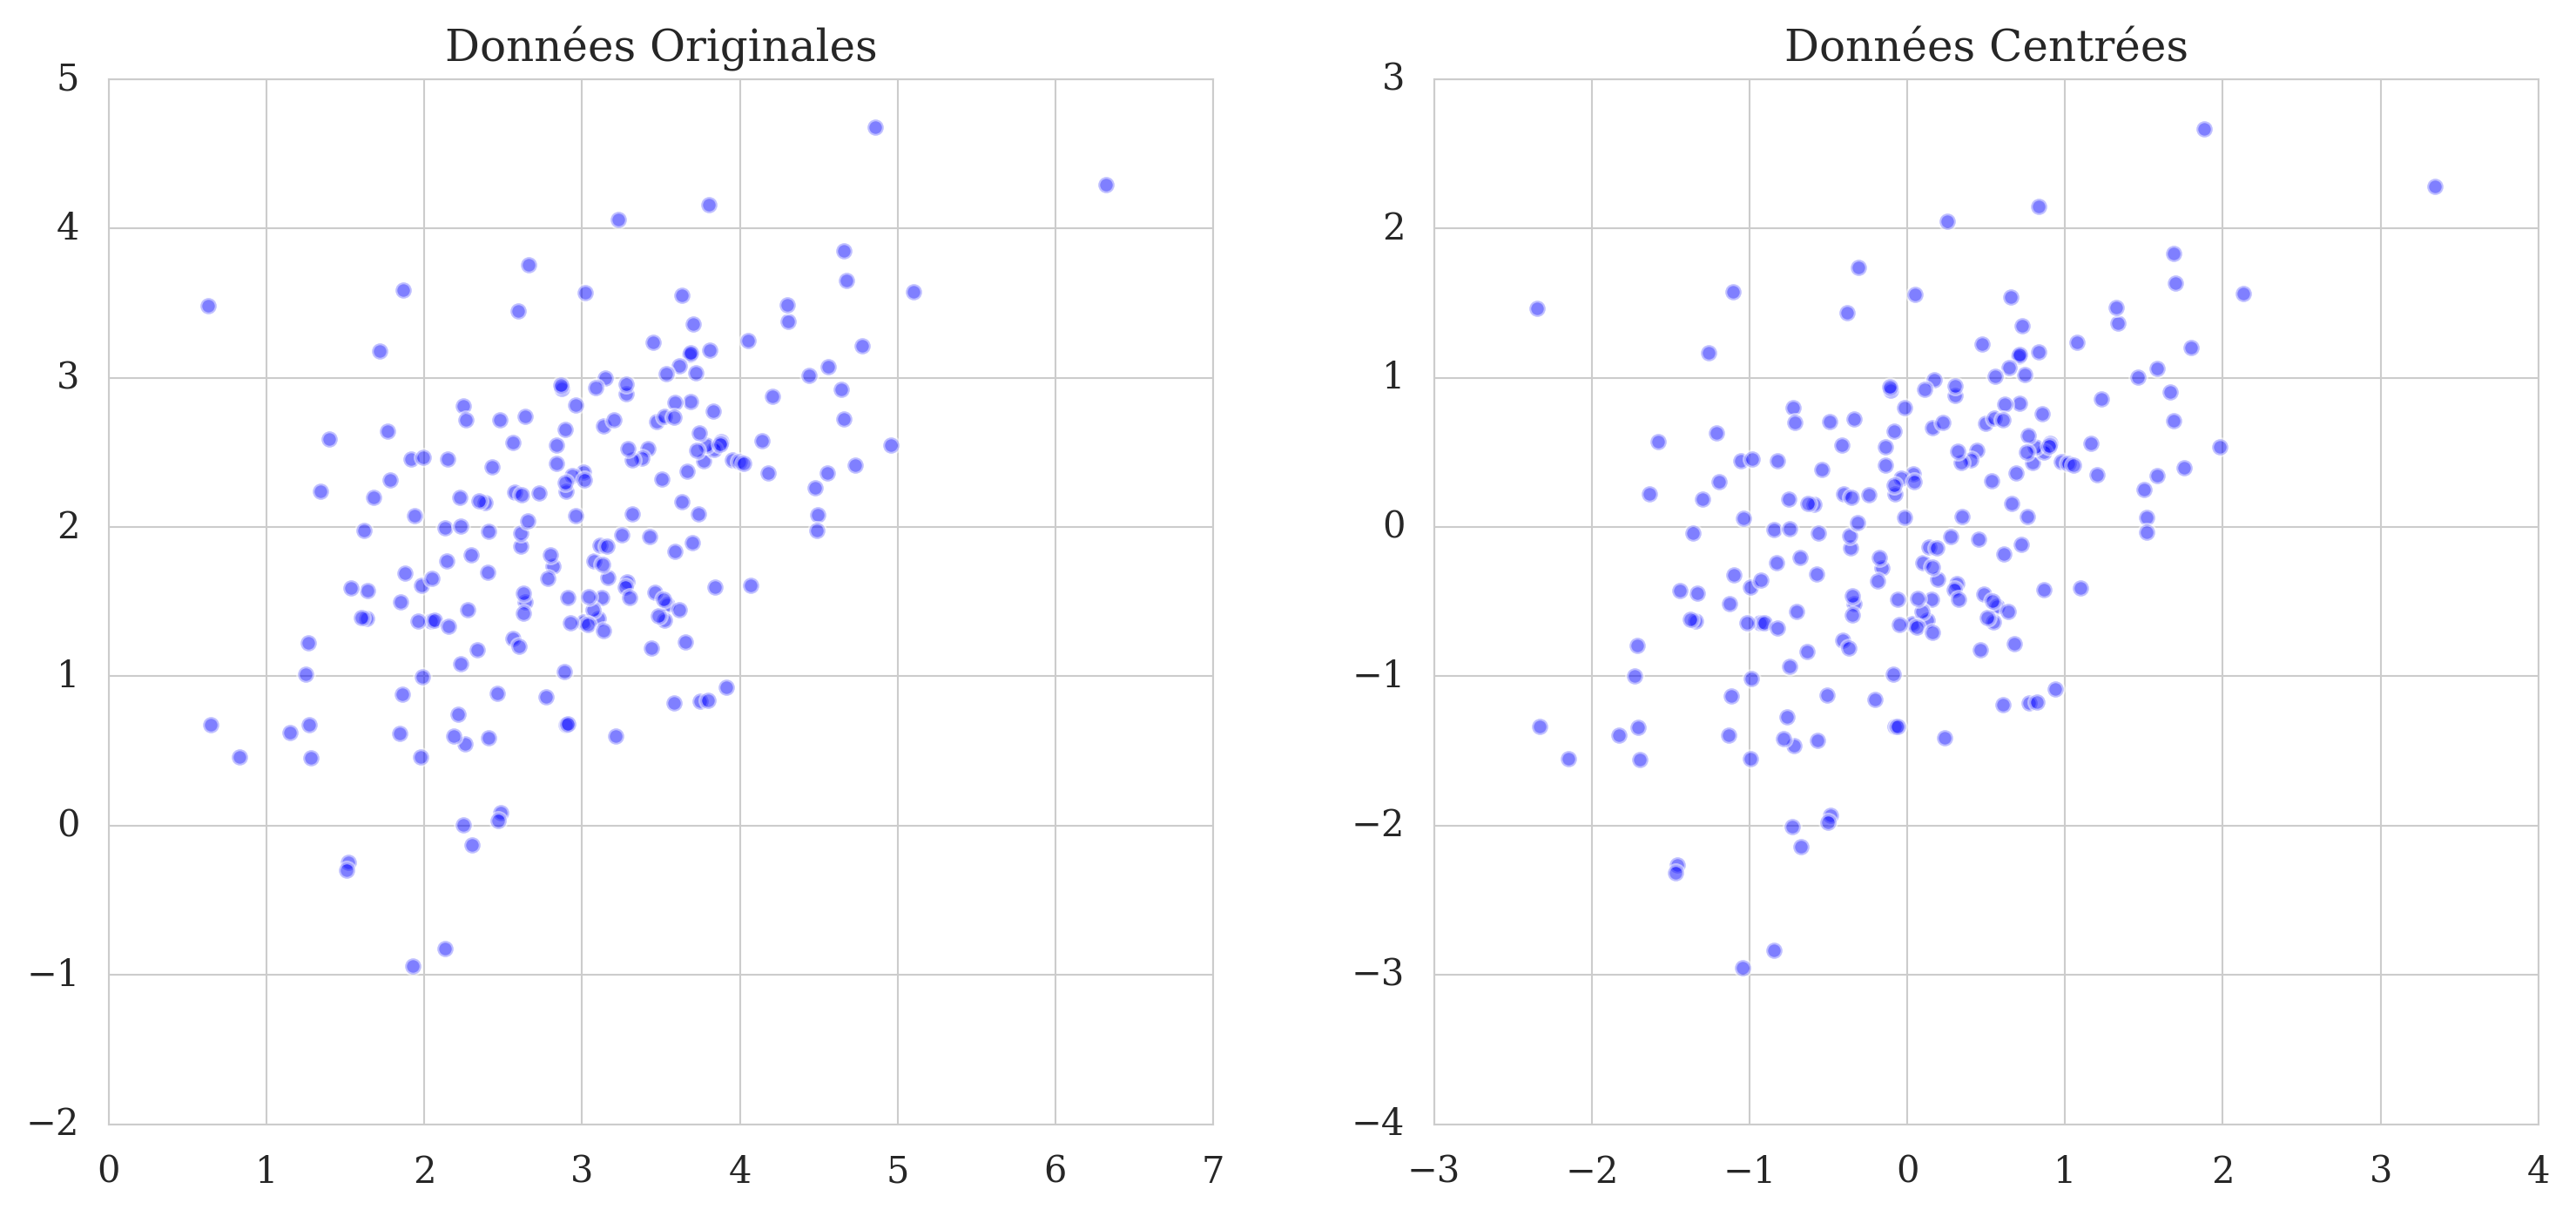
\includegraphics[width=1.1\textwidth]{centrage_normalisation.png}
  \caption{Illustration du centrage et de la normalisation des données.}
  \label{fig:centrage_normalisation_kernel}
\end{figure}
\subsection{Projection des données}

Pour un nouveau point $x$, sa projection sur la $k$-ème composante principale est :

\[
y_k(x) = \sum_{i=1}^n \alpha_i^k k(x_i,x)
\]

où $\alpha^k$ est le $k$-ème vecteur propre normalisé de $\tilde{K}$.

\begin{figure}[H]
  \centering
  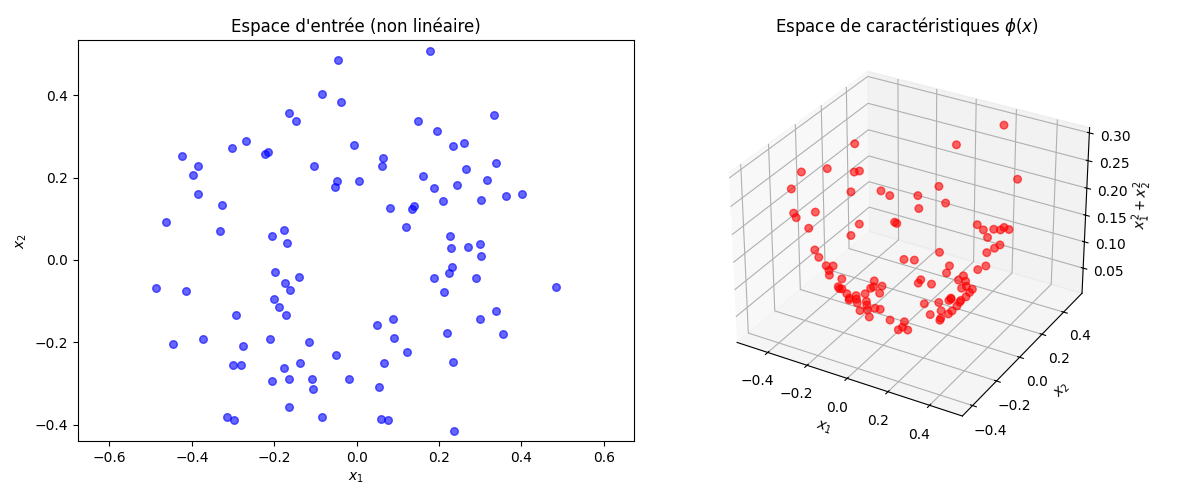
\includegraphics[width=0.8\textwidth]{kernel_mapping.png}
  \caption{Illustration du mapping non linéaire via le kernel trick}
  \label{fig:kernel_mapping}
\end{figure}

\subsection{Complexité et considérations pratiques}

La complexité computationnelle est :
\begin{itemize}
  \item Construction de la matrice de Gram : $O(n^2d)$
  \item Décomposition en valeurs propres : $O(n^3)$
  \item Projection d'un nouveau point : $O(nd)$
\end{itemize}

où $n$ est le nombre d'échantillons et $d$ la dimension d'entrée.

\subsection{Théorème de représentation}

Le théorème de représentation garantit que les vecteurs propres dans $\mathcal{F}$ peuvent s'écrire comme combinaisons linéaires des points projetés :

\[
v = \sum_{i=1}^n \alpha_i \Phi(x_i)
\]

Cette propriété est fondamentale pour l'application pratique du Kernel PCA.

\subsection{Choix du noyau}

Le choix du noyau dépend de la structure des données :
\begin{itemize}
  \item RBF : pour des relations localement lisses
  \item Polynomial : pour des interactions d'ordre supérieur
  \item Sigmoïde : pour des séparations de type perceptron
\end{itemize}

\begin{table}[H]
  \centering
  \begin{tabular}{|l|l|l|}
    \hline
    \textbf{Noyau} & \textbf{Expression} & \textbf{Usage typique} \\
    \hline
    RBF & $\exp(-\gamma\|x-y\|^2)$ & Données continues \\
    Polynomial & $(\langle x,y \rangle + c)^d$ & Features combinatoires \\
    Sigmoïde & $\tanh(\alpha\langle x,y \rangle + c)$ & Classification binaire \\
    \hline
  \end{tabular}
  \caption{Comparaison des noyaux courants}
  \label{tab:kernels}
\end{table} % Add this line to close the table environment

\addcontentsline{toc}{chapter}{Bibliographie}
\begin{thebibliography}{9}
\bibitem{Pearson1901} Pearson, K. (1901). L'analyse des données. Journal de Statistique.
\bibitem{Hotelling1933} Hotelling, H. (1933). Analysis of a complex of statistical variables into principal components. Journal of Educational Psychology.
\bibitem{Jolliffe2002} Jolliffe, I.T. (2002). Principal Component Analysis. Springer.
\bibitem{Bishop2006} Bishop, C.M. (2006). Pattern Recognition and Machine Learning. Springer.
\bibitem{Scholkopf1998} Schölkopf, B., et al. (1998). Nonlinear Component Analysis as a Kernel Eigenvalue Problem. Neural Computation.
\end{thebibliography}

\chapter*{Webographie}
\addcontentsline{toc}{chapter}{Webographie}
\begin{itemize}
  \item \url{https://scikit-learn.org/stable/modules/decomposition.html#pca} - Documentation scikit-learn sur l'ACP
  \item \url{https://stats.stackexchange.com/questions/2691/making-sense-of-principal-component-analysis} - Discussion approfondie sur l'ACP
  \item \url{https://setosa.io/ev/principal-component-analysis/} - Visualisation interactive de l'ACP
  \item \url{https://www.cs.otago.ac.nz/cosc453/student_tutorials/principal_components.pdf} - Tutorial complet sur l'ACP
  \item \url{https://www.kaggle.com/code/arthurtok/interactive-intro-to-dimensionality-reduction} - Exemples pratiques d'ACP
  \item \url{https://www.datasciencecentral.com/principal-component-analysis-for-dimensionality-reduction/} - Applications en data science
  \item \url{https://mathworld.wolfram.com/PrincipalComponentAnalysis.html} - Aspects mathématiques détaillés
  \item \url{https://towardsdatascience.com/a-complete-guide-to-principal-component-analysis-pca-in-machine-learning-664f34fc6a27} - Guide complet
  \item \url{https://en.wikipedia.org/wiki/Principal_component_analysis} - Article Wikipedia détaillé
  \item \url{https://www.youtube.com/watch?v=FgakZw6K1QQ} - Vidéo explicative sur l'ACP
\end{itemize}

\end{document}


